% lecture3.tex -- GENERATED by build_L3.py from L3_numbers.json; do not edit by hand.
\documentclass[10pt,aspectratio=169,t]{beamer}
% =============================================================================
% nn_preamble.tex -- shared Beamer preamble of Neural Networks and Deep Learning (NN)
% Used by every lecture: lectures/Lk/lecturek.tex does
%   \documentclass[10pt,aspectratio=169,t]{beamer}
%   % =============================================================================
% nn_preamble.tex -- shared Beamer preamble of Neural Networks and Deep Learning (NN)
% Used by every lecture: lectures/Lk/lecturek.tex does
%   \documentclass[10pt,aspectratio=169,t]{beamer}
%   % =============================================================================
% nn_preamble.tex -- shared Beamer preamble of Neural Networks and Deep Learning (NN)
% Used by every lecture: lectures/Lk/lecturek.tex does
%   \documentclass[10pt,aspectratio=169,t]{beamer}
%   \input{../common/nn_preamble}
%   \nnlecture{k}{Lecture title}
% Logos live in lectures/common/logos/, charts in lectures/Lk/charts/.
% Do NOT add \hfuzz / \vfuzz / \hbadness here: overfull boxes must be fixed, not hidden.
% =============================================================================

\usetheme{default}
\setbeamersize{text margin left=7mm, text margin right=7mm}

% ---------------------------------------------------------------- packages
\usepackage[utf8]{inputenc}
\usepackage[T1]{fontenc}
\usepackage{lmodern}
\usepackage{amsmath, amssymb}
\usepackage{mathtools}
\usepackage{bm}
\usepackage{tikz}
\usetikzlibrary{arrows.meta, positioning, calc, shapes.misc}
\usepackage{booktabs}
\usepackage{array}
\usepackage{graphicx}
\usepackage{colortbl}
\usepackage{xcolor}
\usepackage{multicol}
\hypersetup{colorlinks=true, linkcolor=MainBlue, urlcolor=MainBlue, citecolor=MainBlue}
\graphicspath{{../common/logos/}}   % charts are included with their language folder: charts/en/, charts/ro/

% ---------------------------------------------------------------- colours
\definecolor{MainBlue}{RGB}{26, 58, 110}
\definecolor{IDAred}{RGB}{205, 0, 0}
\definecolor{DarkGray}{RGB}{51, 51, 51}
\definecolor{FooterGray}{RGB}{100, 100, 100}
\definecolor{BlockGray}{RGB}{236, 238, 242}
\definecolor{KeynoteGray}{RGB}{218, 218, 218}
\definecolor{Crimson}{RGB}{190, 40, 50}
\definecolor{Forest}{RGB}{30, 110, 50}
\definecolor{Bitter}{RGB}{214, 150, 20}
% chart palette (same hex values and order as lectures/common/nn_plot.py SERIES)
\definecolor{Ser1}{HTML}{2A78D6}
\definecolor{Ser2}{HTML}{EB6834}
\definecolor{Ser3}{HTML}{1BAF7A}
\definecolor{Ser4}{HTML}{EDA100}
\definecolor{Ser5}{HTML}{E87BA4}
\definecolor{Ser6}{HTML}{008300}
\definecolor{Ser7}{HTML}{6250D6}
\definecolor{Ser8}{HTML}{E34948}

\setbeamertemplate{background}{%
  \begin{tikzpicture}[remember picture, overlay]
    \shade[shading=axis, shading angle=315, top color=white, bottom color=KeynoteGray]
      (current page.south west) rectangle (current page.north east);
  \end{tikzpicture}}
\setbeamercolor{background canvas}{bg=}
\setbeamercolor{structure}{fg=MainBlue}
\setbeamercolor{normal text}{fg=DarkGray}
\setbeamercolor{title}{fg=IDAred}
\setbeamercolor{frametitle}{fg=IDAred, bg=}
\setbeamercolor{block title}{bg=MainBlue, fg=white}
\setbeamercolor{block body}{bg=BlockGray, fg=DarkGray}
\setbeamercolor{block title alerted}{bg=Crimson, fg=white}
\setbeamercolor{block body alerted}{bg=Crimson!7, fg=DarkGray}
\setbeamercolor{block title example}{bg=Forest, fg=white}
\setbeamercolor{block body example}{bg=Forest!7, fg=DarkGray}
\setbeamercolor{item}{fg=MainBlue}
\setbeamerfont{frametitle}{size=\large, series=\bfseries}
\setbeamerfont{block title}{size=\small, series=\bfseries}
\setbeamertemplate{blocks}[rounded][shadow=false]
\setbeamertemplate{itemize item}{\color{MainBlue}$\boxdot$}
\setbeamertemplate{itemize subitem}{\color{MainBlue}\scriptsize$\blacktriangleright$}
% compact two-level lists: level 1 = main point, level 2 = details (no text outside bullets)
\setbeamerfont{itemize/enumerate subbody}{size=\footnotesize}
\setlength{\leftmargini}{1.1em}
\setlength{\leftmarginii}{1.1em}
\setbeamertemplate{itemize/enumerate body begin}{\setlength{\topsep}{0pt}\setlength{\partopsep}{0pt}\setlength{\parskip}{0pt}}
\setbeamertemplate{itemize/enumerate subbody begin}{\setlength{\topsep}{0pt}\setlength{\partopsep}{0pt}\setlength{\itemsep}{0pt}\vspace{-0.4ex}}

\setbeamertemplate{enumerate item}{\color{MainBlue}\insertenumlabel.}
\setlength{\leftmargini}{1.3em}
\setlength{\leftmarginii}{1.2em}
\setbeamertemplate{navigation symbols}{}
\setbeamertemplate{section in toc}{\color{MainBlue}$\blacktriangleright$~\inserttocsection}
\setbeamertemplate{caption}{\raggedright\insertcaption\par}
% frame subtitle = precise citation line under the claim title (Weron style)
\setbeamerfont{framesubtitle}{size=\footnotesize}
\setbeamercolor{framesubtitle}{fg=FooterGray}
% outline that reappears at every section with the current section highlighted
\setbeamertemplate{section in toc shaded}[default][35]
\setbeamertemplate{subsection in toc shaded}[default][35]
\setbeamertemplate{subsection in toc}{\leavevmode\leftskip=2.2em\color{DarkGray}\small\inserttocsubsection\par}
\AtBeginSection[]{{\begin{frame}{\txtoutline}\vspace{2mm}\small
  \tableofcontents[currentsection,hideothersubsections]\end{frame}}}

% ---------------------------------------------------------------- head and foot
\setbeamertemplate{headline}{%
  \vskip10pt%
  \hbox to \paperwidth{\hskip0.5cm%
    {\small\color{FooterGray}\renewcommand{\hyperlink}[2]{##2}\insertsectionhead}%
    \hfill\textcolor{FooterGray}{\small\insertframenumber}\hskip0.5cm}%
  \vskip4pt{\color{FooterGray}\hrule height 0.4pt}}
% footer as in the other courses (MFM, SFM): course name on the left, small sparkline on the right
\setbeamertemplate{footline}{%
  {\color{FooterGray}\hrule height 0.4pt}\vskip4pt%
  \hbox to \paperwidth{\hskip0.5cm%
    \textcolor{FooterGray}{\small\txtcourse}%
    \hfill\raisebox{-0.1em}{\begin{tikzpicture}[x=0.08em, y=0.08em, line width=0.4pt]
      \draw[FooterGray] (0,3) -- (1,4) -- (2,3.5) -- (3,5) -- (4,4) -- (5,6) -- (6,5.5) -- (7,4) -- (8,5) -- (9,7) -- (10,6) -- (11,5) -- (12,6.5) -- (13,8) -- (14,7) -- (15,6) -- (16,7.5) -- (17,9) -- (18,8) -- (19,7) -- (20,8.5) -- (21,10) -- (22,9) -- (23,8) -- (24,9.5);
    \end{tikzpicture}}\hskip0.5cm}%
  \vskip6pt}

% ---------------------------------------------------------------- title page
\defbeamertemplate*{title page}{nn}[1][]{%
  \vspace{0.15cm}
  \begin{center}
    \href{https://www.ase.ro}{
\includegraphics[height=0.9cm]{ase_logo.png}}\hspace{0.3cm}%
    \href{https://ipe.ro/new}{
\includegraphics[height=0.9cm]{acad_logo.png}}\hspace{0.3cm}%
    \href{https://theida.net}{
\includegraphics[height=0.9cm]{ida_logo.png}}\hspace{0.3cm}%
    \href{https://blockchain-research-center.com}{
\includegraphics[height=0.9cm]{brc_logo.png}}\hspace{0.3cm}%
    \href{https://www.ai4efin.ase.ro}{
\includegraphics[height=0.9cm]{ai4efin_logo.png}}\hspace{0.3cm}%
    \href{https://www.digital-finance-msca.com}{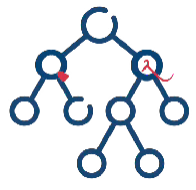
\includegraphics[height=0.9cm]{msca_logo.png}}%
  \end{center}
  \vspace{0.45cm}
  \begin{center}
    \begin{minipage}{0.1\textwidth}\centering
      \href{https://quantlet.com}{
\includegraphics[height=0.9cm]{ql_logo.png}}\end{minipage}%
    \begin{minipage}{0.78\textwidth}\centering
      {\Large\bfseries\usebeamercolor[fg]{title}\inserttitle}\par\vspace{0.25cm}
      {\large\usebeamercolor[fg]{title}\insertsubtitle}\end{minipage}%
    \begin{minipage}{0.1\textwidth}\centering
      \href{https://quantinar.com}{
\includegraphics[height=0.9cm]{qr_logo.png}}\end{minipage}
  \end{center}
  \vfill
  \hspace{0.4cm}{\bfseries\insertauthor}\par\vspace{0.12cm}
  \hspace{0.4cm}\begin{minipage}[t]{0.92\textwidth}\raggedright\footnotesize\insertinstitute\end{minipage}
  \par\vspace{0.4cm}}

% ---------------------------------------------------------------- lecture metadata
\newcommand{\nnshort}{}
\newcommand{\nnnb}{notebooks}
\newcommand{\nnrepo}{https://github.com/danpele/NEURAL_BIZ/tree/main}
% language-dependent labels (English default; \nnromanian switches to Romanian, call it before \nnlecture)
\newcommand{\txtcourse}{Neural Networks and Deep Learning}
\newcommand{\txtlecture}{Lecture}
\newcommand{\txtoutline}{Outline}
\newcommand{\txtintuition}{In one sentence:}
\newcommand{\txtjob}{In practice:}
\newcommand{\txttry}{Experiment yourself:}
\newcommand{\txtwhere}{where}
\newcommand{\txtsim}{SIMULATED DATA (teaching illustration)}
\newcommand{\txtnbsuffix}{}
\newcommand{\txtinstitute}{Bucharest University of Economic Studies (ASE), Department of Statistics and Econometrics\\
    Romanian Academy, Institute for Economic Forecasting (IPE)\\
    IDA Institute Digital Assets \textbullet\ AI4EFin \textbullet\ MSCA Digital Finance}
\newcommand{\nnromanian}{%
  \renewcommand{\txtcourse}{Rețele neuronale și deep learning}%
  \renewcommand{\txtlecture}{Cursul}%
  \renewcommand{\txtoutline}{Cuprins}%
  \renewcommand{\txtintuition}{Pe scurt:}%
  \renewcommand{\txtjob}{În practică:}%
  \renewcommand{\txttry}{Exercițiu practic:}%
  \renewcommand{\txtwhere}{unde}%
  \renewcommand{\txtsim}{DATE SIMULATE (doar pentru ilustrare)}%
  \renewcommand{\txtnbsuffix}{\string_ro}%
  \renewcommand{\txtinstitute}{Academia de Studii Economice din București (ASE), Departamentul de Statistică și Econometrie\\
    Academia Română, Institutul de Prognoză Economică (IPE)\\
    IDA Institute Digital Assets \textbullet\ AI4EFin \textbullet\ MSCA Digital Finance}}
\newcommand{\nnlecture}[2]{%
  \renewcommand{\nnshort}{\txtlecture\ #1}%
  \renewcommand{\nnnb}{notebooks/L#1\string_notebook\txtnbsuffix.ipynb}%
  \title[NN]{\txtcourse}%
  \subtitle{\txtlecture\ #1: #2}%
  \author{Prof.\ dr.\ Daniel Traian PELE}%
  \institute{\txtinstitute}%
  \date{}}

% ---------------------------------------------------------------- teaching blocks (one message per frame)
% \intuition{one plain sentence}  ->  formula with every symbol defined  ->  real-data example  ->  \manager{one line}
\newcommand{\intuition}[1]{\begin{itemize}\item {\color{MainBlue}\textbf{\txtintuition}}~#1\end{itemize}\vspace{0.6mm}}
\newcommand{\manager}[1]{\colorbox{Forest!10}{\parbox{\dimexpr\linewidth-2\fboxsep\relax}{\footnotesize
  \begin{itemize}\setlength{\itemsep}{0pt}\item \textbf{\color{Forest}\txtjob}~#1\end{itemize}}}}
% Experiment yourself: pointer to the matching notebook section
\newcommand{\tryit}[1]{{\scriptsize\href{\nnrepo/\nnnb}{%
  \raisebox{-0.15em}{
\includegraphics[height=0.85em]{ql_logo.png}}\,\textbf{\txttry}~\color{MainBlue}#1}}}
% bottom row: manager line (left) + experiment pointer (right), pinned to the bottom of the frame
\newcommand{\bottomrow}[2]{\par\vfill\noindent\begin{minipage}[b]{0.72\linewidth}#1\end{minipage}\hfill
  \begin{minipage}[b]{0.26\linewidth}\raggedleft #2\end{minipage}\par\vspace{0.5mm}}
\newcommand{\where}[1]{{\footnotesize\textbf{\txtwhere}~#1\par}}

% ---------------------------------------------------------------- helpers
% chart source line under a figure: \chartsource{Source ...; period ...}
\newcommand{\chartsource}[1]{\par\vspace{1pt}{\scriptsize\color{FooterGray}#1\par}}
% link to code: \quantlet{label}{path inside the repo}
\newcommand{\quantlet}[2]{\par\vspace{1pt}\hfill\href{\nnrepo/#2}{%
  \raisebox{-0.15em}{
\includegraphics[height=0.75em]{ql_logo.png}}\textcolor{MainBlue}{\scriptsize\ #1}}}
% inline Quantlet link for the bottom-right corner of a frame: \qlink{label}{path inside the repo}
\newcommand{\qlink}[2]{{\scriptsize\href{\nnrepo/#2}{\raisebox{-0.15em}{
\includegraphics[height=0.85em]{ql_logo.png}}\,\textcolor{MainBlue}{#1}}}}
\newcommand{\simlabel}{\colorbox{Crimson!12}{\scriptsize\bfseries\color{Crimson}\txtsim}}
\newcommand{\E}{\mathbb{E}}
\newcommand{\Var}{\operatorname{Var}}
\newcommand{\Cov}{\operatorname{Cov}}
\newcommand{\Corr}{\operatorname{Corr}}
\newcommand{\asinh}{\operatorname{asinh}}
\newcommand{\iid}{\overset{\text{i.i.d.}}{\sim}}
\newcommand{\EUR}{EUR}
% deep-learning notation (Bishop & Bishop, 2024): vectors bold lower case, matrices bold upper case
\newcommand{\R}{\mathbb{R}}
\newcommand{\vx}{\mathbf{x}}
\newcommand{\vy}{\mathbf{y}}
\newcommand{\vz}{\mathbf{z}}
\newcommand{\vh}{\mathbf{h}}
\newcommand{\vw}{\mathbf{w}}
\newcommand{\vb}{\mathbf{b}}
\newcommand{\mW}{\mathbf{W}}
\newcommand{\mX}{\mathbf{X}}
\newcommand{\btheta}{\boldsymbol{\theta}}
\newcommand{\loss}{\mathcal{L}}
\newcommand{\dataset}{\mathcal{D}}
\DeclareMathOperator*{\argmin}{arg\,min}
\DeclareMathOperator*{\argmax}{arg\,max}
\DeclareMathOperator{\softmax}{softmax}
\DeclareMathOperator{\ReLU}{ReLU}
\DeclareMathOperator{\sigm}{\sigma}

%   \nnlecture{k}{Lecture title}
% Logos live in lectures/common/logos/, charts in lectures/Lk/charts/.
% Do NOT add \hfuzz / \vfuzz / \hbadness here: overfull boxes must be fixed, not hidden.
% =============================================================================

\usetheme{default}
\setbeamersize{text margin left=7mm, text margin right=7mm}

% ---------------------------------------------------------------- packages
\usepackage[utf8]{inputenc}
\usepackage[T1]{fontenc}
\usepackage{lmodern}
\usepackage{amsmath, amssymb}
\usepackage{mathtools}
\usepackage{bm}
\usepackage{tikz}
\usetikzlibrary{arrows.meta, positioning, calc, shapes.misc}
\usepackage{booktabs}
\usepackage{array}
\usepackage{graphicx}
\usepackage{colortbl}
\usepackage{xcolor}
\usepackage{multicol}
\hypersetup{colorlinks=true, linkcolor=MainBlue, urlcolor=MainBlue, citecolor=MainBlue}
\graphicspath{{../common/logos/}}   % charts are included with their language folder: charts/en/, charts/ro/

% ---------------------------------------------------------------- colours
\definecolor{MainBlue}{RGB}{26, 58, 110}
\definecolor{IDAred}{RGB}{205, 0, 0}
\definecolor{DarkGray}{RGB}{51, 51, 51}
\definecolor{FooterGray}{RGB}{100, 100, 100}
\definecolor{BlockGray}{RGB}{236, 238, 242}
\definecolor{KeynoteGray}{RGB}{218, 218, 218}
\definecolor{Crimson}{RGB}{190, 40, 50}
\definecolor{Forest}{RGB}{30, 110, 50}
\definecolor{Bitter}{RGB}{214, 150, 20}
% chart palette (same hex values and order as lectures/common/nn_plot.py SERIES)
\definecolor{Ser1}{HTML}{2A78D6}
\definecolor{Ser2}{HTML}{EB6834}
\definecolor{Ser3}{HTML}{1BAF7A}
\definecolor{Ser4}{HTML}{EDA100}
\definecolor{Ser5}{HTML}{E87BA4}
\definecolor{Ser6}{HTML}{008300}
\definecolor{Ser7}{HTML}{6250D6}
\definecolor{Ser8}{HTML}{E34948}

\setbeamertemplate{background}{%
  \begin{tikzpicture}[remember picture, overlay]
    \shade[shading=axis, shading angle=315, top color=white, bottom color=KeynoteGray]
      (current page.south west) rectangle (current page.north east);
  \end{tikzpicture}}
\setbeamercolor{background canvas}{bg=}
\setbeamercolor{structure}{fg=MainBlue}
\setbeamercolor{normal text}{fg=DarkGray}
\setbeamercolor{title}{fg=IDAred}
\setbeamercolor{frametitle}{fg=IDAred, bg=}
\setbeamercolor{block title}{bg=MainBlue, fg=white}
\setbeamercolor{block body}{bg=BlockGray, fg=DarkGray}
\setbeamercolor{block title alerted}{bg=Crimson, fg=white}
\setbeamercolor{block body alerted}{bg=Crimson!7, fg=DarkGray}
\setbeamercolor{block title example}{bg=Forest, fg=white}
\setbeamercolor{block body example}{bg=Forest!7, fg=DarkGray}
\setbeamercolor{item}{fg=MainBlue}
\setbeamerfont{frametitle}{size=\large, series=\bfseries}
\setbeamerfont{block title}{size=\small, series=\bfseries}
\setbeamertemplate{blocks}[rounded][shadow=false]
\setbeamertemplate{itemize item}{\color{MainBlue}$\boxdot$}
\setbeamertemplate{itemize subitem}{\color{MainBlue}\scriptsize$\blacktriangleright$}
% compact two-level lists: level 1 = main point, level 2 = details (no text outside bullets)
\setbeamerfont{itemize/enumerate subbody}{size=\footnotesize}
\setlength{\leftmargini}{1.1em}
\setlength{\leftmarginii}{1.1em}
\setbeamertemplate{itemize/enumerate body begin}{\setlength{\topsep}{0pt}\setlength{\partopsep}{0pt}\setlength{\parskip}{0pt}}
\setbeamertemplate{itemize/enumerate subbody begin}{\setlength{\topsep}{0pt}\setlength{\partopsep}{0pt}\setlength{\itemsep}{0pt}\vspace{-0.4ex}}

\setbeamertemplate{enumerate item}{\color{MainBlue}\insertenumlabel.}
\setlength{\leftmargini}{1.3em}
\setlength{\leftmarginii}{1.2em}
\setbeamertemplate{navigation symbols}{}
\setbeamertemplate{section in toc}{\color{MainBlue}$\blacktriangleright$~\inserttocsection}
\setbeamertemplate{caption}{\raggedright\insertcaption\par}
% frame subtitle = precise citation line under the claim title (Weron style)
\setbeamerfont{framesubtitle}{size=\footnotesize}
\setbeamercolor{framesubtitle}{fg=FooterGray}
% outline that reappears at every section with the current section highlighted
\setbeamertemplate{section in toc shaded}[default][35]
\setbeamertemplate{subsection in toc shaded}[default][35]
\setbeamertemplate{subsection in toc}{\leavevmode\leftskip=2.2em\color{DarkGray}\small\inserttocsubsection\par}
\AtBeginSection[]{{\begin{frame}{\txtoutline}\vspace{2mm}\small
  \tableofcontents[currentsection,hideothersubsections]\end{frame}}}

% ---------------------------------------------------------------- head and foot
\setbeamertemplate{headline}{%
  \vskip10pt%
  \hbox to \paperwidth{\hskip0.5cm%
    {\small\color{FooterGray}\renewcommand{\hyperlink}[2]{##2}\insertsectionhead}%
    \hfill\textcolor{FooterGray}{\small\insertframenumber}\hskip0.5cm}%
  \vskip4pt{\color{FooterGray}\hrule height 0.4pt}}
% footer as in the other courses (MFM, SFM): course name on the left, small sparkline on the right
\setbeamertemplate{footline}{%
  {\color{FooterGray}\hrule height 0.4pt}\vskip4pt%
  \hbox to \paperwidth{\hskip0.5cm%
    \textcolor{FooterGray}{\small\txtcourse}%
    \hfill\raisebox{-0.1em}{\begin{tikzpicture}[x=0.08em, y=0.08em, line width=0.4pt]
      \draw[FooterGray] (0,3) -- (1,4) -- (2,3.5) -- (3,5) -- (4,4) -- (5,6) -- (6,5.5) -- (7,4) -- (8,5) -- (9,7) -- (10,6) -- (11,5) -- (12,6.5) -- (13,8) -- (14,7) -- (15,6) -- (16,7.5) -- (17,9) -- (18,8) -- (19,7) -- (20,8.5) -- (21,10) -- (22,9) -- (23,8) -- (24,9.5);
    \end{tikzpicture}}\hskip0.5cm}%
  \vskip6pt}

% ---------------------------------------------------------------- title page
\defbeamertemplate*{title page}{nn}[1][]{%
  \vspace{0.15cm}
  \begin{center}
    \href{https://www.ase.ro}{
\includegraphics[height=0.9cm]{ase_logo.png}}\hspace{0.3cm}%
    \href{https://ipe.ro/new}{
\includegraphics[height=0.9cm]{acad_logo.png}}\hspace{0.3cm}%
    \href{https://theida.net}{
\includegraphics[height=0.9cm]{ida_logo.png}}\hspace{0.3cm}%
    \href{https://blockchain-research-center.com}{
\includegraphics[height=0.9cm]{brc_logo.png}}\hspace{0.3cm}%
    \href{https://www.ai4efin.ase.ro}{
\includegraphics[height=0.9cm]{ai4efin_logo.png}}\hspace{0.3cm}%
    \href{https://www.digital-finance-msca.com}{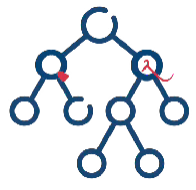
\includegraphics[height=0.9cm]{msca_logo.png}}%
  \end{center}
  \vspace{0.45cm}
  \begin{center}
    \begin{minipage}{0.1\textwidth}\centering
      \href{https://quantlet.com}{
\includegraphics[height=0.9cm]{ql_logo.png}}\end{minipage}%
    \begin{minipage}{0.78\textwidth}\centering
      {\Large\bfseries\usebeamercolor[fg]{title}\inserttitle}\par\vspace{0.25cm}
      {\large\usebeamercolor[fg]{title}\insertsubtitle}\end{minipage}%
    \begin{minipage}{0.1\textwidth}\centering
      \href{https://quantinar.com}{
\includegraphics[height=0.9cm]{qr_logo.png}}\end{minipage}
  \end{center}
  \vfill
  \hspace{0.4cm}{\bfseries\insertauthor}\par\vspace{0.12cm}
  \hspace{0.4cm}\begin{minipage}[t]{0.92\textwidth}\raggedright\footnotesize\insertinstitute\end{minipage}
  \par\vspace{0.4cm}}

% ---------------------------------------------------------------- lecture metadata
\newcommand{\nnshort}{}
\newcommand{\nnnb}{notebooks}
\newcommand{\nnrepo}{https://github.com/danpele/NEURAL_BIZ/tree/main}
% language-dependent labels (English default; \nnromanian switches to Romanian, call it before \nnlecture)
\newcommand{\txtcourse}{Neural Networks and Deep Learning}
\newcommand{\txtlecture}{Lecture}
\newcommand{\txtoutline}{Outline}
\newcommand{\txtintuition}{In one sentence:}
\newcommand{\txtjob}{In practice:}
\newcommand{\txttry}{Experiment yourself:}
\newcommand{\txtwhere}{where}
\newcommand{\txtsim}{SIMULATED DATA (teaching illustration)}
\newcommand{\txtnbsuffix}{}
\newcommand{\txtinstitute}{Bucharest University of Economic Studies (ASE), Department of Statistics and Econometrics\\
    Romanian Academy, Institute for Economic Forecasting (IPE)\\
    IDA Institute Digital Assets \textbullet\ AI4EFin \textbullet\ MSCA Digital Finance}
\newcommand{\nnromanian}{%
  \renewcommand{\txtcourse}{Rețele neuronale și deep learning}%
  \renewcommand{\txtlecture}{Cursul}%
  \renewcommand{\txtoutline}{Cuprins}%
  \renewcommand{\txtintuition}{Pe scurt:}%
  \renewcommand{\txtjob}{În practică:}%
  \renewcommand{\txttry}{Exercițiu practic:}%
  \renewcommand{\txtwhere}{unde}%
  \renewcommand{\txtsim}{DATE SIMULATE (doar pentru ilustrare)}%
  \renewcommand{\txtnbsuffix}{\string_ro}%
  \renewcommand{\txtinstitute}{Academia de Studii Economice din București (ASE), Departamentul de Statistică și Econometrie\\
    Academia Română, Institutul de Prognoză Economică (IPE)\\
    IDA Institute Digital Assets \textbullet\ AI4EFin \textbullet\ MSCA Digital Finance}}
\newcommand{\nnlecture}[2]{%
  \renewcommand{\nnshort}{\txtlecture\ #1}%
  \renewcommand{\nnnb}{notebooks/L#1\string_notebook\txtnbsuffix.ipynb}%
  \title[NN]{\txtcourse}%
  \subtitle{\txtlecture\ #1: #2}%
  \author{Prof.\ dr.\ Daniel Traian PELE}%
  \institute{\txtinstitute}%
  \date{}}

% ---------------------------------------------------------------- teaching blocks (one message per frame)
% \intuition{one plain sentence}  ->  formula with every symbol defined  ->  real-data example  ->  \manager{one line}
\newcommand{\intuition}[1]{\begin{itemize}\item {\color{MainBlue}\textbf{\txtintuition}}~#1\end{itemize}\vspace{0.6mm}}
\newcommand{\manager}[1]{\colorbox{Forest!10}{\parbox{\dimexpr\linewidth-2\fboxsep\relax}{\footnotesize
  \begin{itemize}\setlength{\itemsep}{0pt}\item \textbf{\color{Forest}\txtjob}~#1\end{itemize}}}}
% Experiment yourself: pointer to the matching notebook section
\newcommand{\tryit}[1]{{\scriptsize\href{\nnrepo/\nnnb}{%
  \raisebox{-0.15em}{
\includegraphics[height=0.85em]{ql_logo.png}}\,\textbf{\txttry}~\color{MainBlue}#1}}}
% bottom row: manager line (left) + experiment pointer (right), pinned to the bottom of the frame
\newcommand{\bottomrow}[2]{\par\vfill\noindent\begin{minipage}[b]{0.72\linewidth}#1\end{minipage}\hfill
  \begin{minipage}[b]{0.26\linewidth}\raggedleft #2\end{minipage}\par\vspace{0.5mm}}
\newcommand{\where}[1]{{\footnotesize\textbf{\txtwhere}~#1\par}}

% ---------------------------------------------------------------- helpers
% chart source line under a figure: \chartsource{Source ...; period ...}
\newcommand{\chartsource}[1]{\par\vspace{1pt}{\scriptsize\color{FooterGray}#1\par}}
% link to code: \quantlet{label}{path inside the repo}
\newcommand{\quantlet}[2]{\par\vspace{1pt}\hfill\href{\nnrepo/#2}{%
  \raisebox{-0.15em}{
\includegraphics[height=0.75em]{ql_logo.png}}\textcolor{MainBlue}{\scriptsize\ #1}}}
% inline Quantlet link for the bottom-right corner of a frame: \qlink{label}{path inside the repo}
\newcommand{\qlink}[2]{{\scriptsize\href{\nnrepo/#2}{\raisebox{-0.15em}{
\includegraphics[height=0.85em]{ql_logo.png}}\,\textcolor{MainBlue}{#1}}}}
\newcommand{\simlabel}{\colorbox{Crimson!12}{\scriptsize\bfseries\color{Crimson}\txtsim}}
\newcommand{\E}{\mathbb{E}}
\newcommand{\Var}{\operatorname{Var}}
\newcommand{\Cov}{\operatorname{Cov}}
\newcommand{\Corr}{\operatorname{Corr}}
\newcommand{\asinh}{\operatorname{asinh}}
\newcommand{\iid}{\overset{\text{i.i.d.}}{\sim}}
\newcommand{\EUR}{EUR}
% deep-learning notation (Bishop & Bishop, 2024): vectors bold lower case, matrices bold upper case
\newcommand{\R}{\mathbb{R}}
\newcommand{\vx}{\mathbf{x}}
\newcommand{\vy}{\mathbf{y}}
\newcommand{\vz}{\mathbf{z}}
\newcommand{\vh}{\mathbf{h}}
\newcommand{\vw}{\mathbf{w}}
\newcommand{\vb}{\mathbf{b}}
\newcommand{\mW}{\mathbf{W}}
\newcommand{\mX}{\mathbf{X}}
\newcommand{\btheta}{\boldsymbol{\theta}}
\newcommand{\loss}{\mathcal{L}}
\newcommand{\dataset}{\mathcal{D}}
\DeclareMathOperator*{\argmin}{arg\,min}
\DeclareMathOperator*{\argmax}{arg\,max}
\DeclareMathOperator{\softmax}{softmax}
\DeclareMathOperator{\ReLU}{ReLU}
\DeclareMathOperator{\sigm}{\sigma}

%   \nnlecture{k}{Lecture title}
% Logos live in lectures/common/logos/, charts in lectures/Lk/charts/.
% Do NOT add \hfuzz / \vfuzz / \hbadness here: overfull boxes must be fixed, not hidden.
% =============================================================================

\usetheme{default}
\setbeamersize{text margin left=7mm, text margin right=7mm}

% ---------------------------------------------------------------- packages
\usepackage[utf8]{inputenc}
\usepackage[T1]{fontenc}
\usepackage{lmodern}
\usepackage{amsmath, amssymb}
\usepackage{mathtools}
\usepackage{bm}
\usepackage{tikz}
\usetikzlibrary{arrows.meta, positioning, calc, shapes.misc}
\usepackage{booktabs}
\usepackage{array}
\usepackage{graphicx}
\usepackage{colortbl}
\usepackage{xcolor}
\usepackage{multicol}
\hypersetup{colorlinks=true, linkcolor=MainBlue, urlcolor=MainBlue, citecolor=MainBlue}
\graphicspath{{../common/logos/}}   % charts are included with their language folder: charts/en/, charts/ro/

% ---------------------------------------------------------------- colours
\definecolor{MainBlue}{RGB}{26, 58, 110}
\definecolor{IDAred}{RGB}{205, 0, 0}
\definecolor{DarkGray}{RGB}{51, 51, 51}
\definecolor{FooterGray}{RGB}{100, 100, 100}
\definecolor{BlockGray}{RGB}{236, 238, 242}
\definecolor{KeynoteGray}{RGB}{218, 218, 218}
\definecolor{Crimson}{RGB}{190, 40, 50}
\definecolor{Forest}{RGB}{30, 110, 50}
\definecolor{Bitter}{RGB}{214, 150, 20}
% chart palette (same hex values and order as lectures/common/nn_plot.py SERIES)
\definecolor{Ser1}{HTML}{2A78D6}
\definecolor{Ser2}{HTML}{EB6834}
\definecolor{Ser3}{HTML}{1BAF7A}
\definecolor{Ser4}{HTML}{EDA100}
\definecolor{Ser5}{HTML}{E87BA4}
\definecolor{Ser6}{HTML}{008300}
\definecolor{Ser7}{HTML}{6250D6}
\definecolor{Ser8}{HTML}{E34948}

\setbeamertemplate{background}{%
  \begin{tikzpicture}[remember picture, overlay]
    \shade[shading=axis, shading angle=315, top color=white, bottom color=KeynoteGray]
      (current page.south west) rectangle (current page.north east);
  \end{tikzpicture}}
\setbeamercolor{background canvas}{bg=}
\setbeamercolor{structure}{fg=MainBlue}
\setbeamercolor{normal text}{fg=DarkGray}
\setbeamercolor{title}{fg=IDAred}
\setbeamercolor{frametitle}{fg=IDAred, bg=}
\setbeamercolor{block title}{bg=MainBlue, fg=white}
\setbeamercolor{block body}{bg=BlockGray, fg=DarkGray}
\setbeamercolor{block title alerted}{bg=Crimson, fg=white}
\setbeamercolor{block body alerted}{bg=Crimson!7, fg=DarkGray}
\setbeamercolor{block title example}{bg=Forest, fg=white}
\setbeamercolor{block body example}{bg=Forest!7, fg=DarkGray}
\setbeamercolor{item}{fg=MainBlue}
\setbeamerfont{frametitle}{size=\large, series=\bfseries}
\setbeamerfont{block title}{size=\small, series=\bfseries}
\setbeamertemplate{blocks}[rounded][shadow=false]
\setbeamertemplate{itemize item}{\color{MainBlue}$\boxdot$}
\setbeamertemplate{itemize subitem}{\color{MainBlue}\scriptsize$\blacktriangleright$}
% compact two-level lists: level 1 = main point, level 2 = details (no text outside bullets)
\setbeamerfont{itemize/enumerate subbody}{size=\footnotesize}
\setlength{\leftmargini}{1.1em}
\setlength{\leftmarginii}{1.1em}
\setbeamertemplate{itemize/enumerate body begin}{\setlength{\topsep}{0pt}\setlength{\partopsep}{0pt}\setlength{\parskip}{0pt}}
\setbeamertemplate{itemize/enumerate subbody begin}{\setlength{\topsep}{0pt}\setlength{\partopsep}{0pt}\setlength{\itemsep}{0pt}\vspace{-0.4ex}}

\setbeamertemplate{enumerate item}{\color{MainBlue}\insertenumlabel.}
\setlength{\leftmargini}{1.3em}
\setlength{\leftmarginii}{1.2em}
\setbeamertemplate{navigation symbols}{}
\setbeamertemplate{section in toc}{\color{MainBlue}$\blacktriangleright$~\inserttocsection}
\setbeamertemplate{caption}{\raggedright\insertcaption\par}
% frame subtitle = precise citation line under the claim title (Weron style)
\setbeamerfont{framesubtitle}{size=\footnotesize}
\setbeamercolor{framesubtitle}{fg=FooterGray}
% outline that reappears at every section with the current section highlighted
\setbeamertemplate{section in toc shaded}[default][35]
\setbeamertemplate{subsection in toc shaded}[default][35]
\setbeamertemplate{subsection in toc}{\leavevmode\leftskip=2.2em\color{DarkGray}\small\inserttocsubsection\par}
\AtBeginSection[]{{\begin{frame}{\txtoutline}\vspace{2mm}\small
  \tableofcontents[currentsection,hideothersubsections]\end{frame}}}

% ---------------------------------------------------------------- head and foot
\setbeamertemplate{headline}{%
  \vskip10pt%
  \hbox to \paperwidth{\hskip0.5cm%
    {\small\color{FooterGray}\renewcommand{\hyperlink}[2]{##2}\insertsectionhead}%
    \hfill\textcolor{FooterGray}{\small\insertframenumber}\hskip0.5cm}%
  \vskip4pt{\color{FooterGray}\hrule height 0.4pt}}
% footer as in the other courses (MFM, SFM): course name on the left, small sparkline on the right
\setbeamertemplate{footline}{%
  {\color{FooterGray}\hrule height 0.4pt}\vskip4pt%
  \hbox to \paperwidth{\hskip0.5cm%
    \textcolor{FooterGray}{\small\txtcourse}%
    \hfill\raisebox{-0.1em}{\begin{tikzpicture}[x=0.08em, y=0.08em, line width=0.4pt]
      \draw[FooterGray] (0,3) -- (1,4) -- (2,3.5) -- (3,5) -- (4,4) -- (5,6) -- (6,5.5) -- (7,4) -- (8,5) -- (9,7) -- (10,6) -- (11,5) -- (12,6.5) -- (13,8) -- (14,7) -- (15,6) -- (16,7.5) -- (17,9) -- (18,8) -- (19,7) -- (20,8.5) -- (21,10) -- (22,9) -- (23,8) -- (24,9.5);
    \end{tikzpicture}}\hskip0.5cm}%
  \vskip6pt}

% ---------------------------------------------------------------- title page
\defbeamertemplate*{title page}{nn}[1][]{%
  \vspace{0.15cm}
  \begin{center}
    \href{https://www.ase.ro}{
\includegraphics[height=0.9cm]{ase_logo.png}}\hspace{0.3cm}%
    \href{https://ipe.ro/new}{
\includegraphics[height=0.9cm]{acad_logo.png}}\hspace{0.3cm}%
    \href{https://theida.net}{
\includegraphics[height=0.9cm]{ida_logo.png}}\hspace{0.3cm}%
    \href{https://blockchain-research-center.com}{
\includegraphics[height=0.9cm]{brc_logo.png}}\hspace{0.3cm}%
    \href{https://www.ai4efin.ase.ro}{
\includegraphics[height=0.9cm]{ai4efin_logo.png}}\hspace{0.3cm}%
    \href{https://www.digital-finance-msca.com}{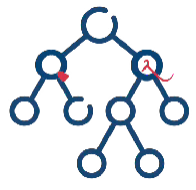
\includegraphics[height=0.9cm]{msca_logo.png}}%
  \end{center}
  \vspace{0.45cm}
  \begin{center}
    \begin{minipage}{0.1\textwidth}\centering
      \href{https://quantlet.com}{
\includegraphics[height=0.9cm]{ql_logo.png}}\end{minipage}%
    \begin{minipage}{0.78\textwidth}\centering
      {\Large\bfseries\usebeamercolor[fg]{title}\inserttitle}\par\vspace{0.25cm}
      {\large\usebeamercolor[fg]{title}\insertsubtitle}\end{minipage}%
    \begin{minipage}{0.1\textwidth}\centering
      \href{https://quantinar.com}{
\includegraphics[height=0.9cm]{qr_logo.png}}\end{minipage}
  \end{center}
  \vfill
  \hspace{0.4cm}{\bfseries\insertauthor}\par\vspace{0.12cm}
  \hspace{0.4cm}\begin{minipage}[t]{0.92\textwidth}\raggedright\footnotesize\insertinstitute\end{minipage}
  \par\vspace{0.4cm}}

% ---------------------------------------------------------------- lecture metadata
\newcommand{\nnshort}{}
\newcommand{\nnnb}{notebooks}
\newcommand{\nnrepo}{https://github.com/danpele/NEURAL_BIZ/tree/main}
% language-dependent labels (English default; \nnromanian switches to Romanian, call it before \nnlecture)
\newcommand{\txtcourse}{Neural Networks and Deep Learning}
\newcommand{\txtlecture}{Lecture}
\newcommand{\txtoutline}{Outline}
\newcommand{\txtintuition}{In one sentence:}
\newcommand{\txtjob}{In practice:}
\newcommand{\txttry}{Experiment yourself:}
\newcommand{\txtwhere}{where}
\newcommand{\txtsim}{SIMULATED DATA (teaching illustration)}
\newcommand{\txtnbsuffix}{}
\newcommand{\txtinstitute}{Bucharest University of Economic Studies (ASE), Department of Statistics and Econometrics\\
    Romanian Academy, Institute for Economic Forecasting (IPE)\\
    IDA Institute Digital Assets \textbullet\ AI4EFin \textbullet\ MSCA Digital Finance}
\newcommand{\nnromanian}{%
  \renewcommand{\txtcourse}{Rețele neuronale și deep learning}%
  \renewcommand{\txtlecture}{Cursul}%
  \renewcommand{\txtoutline}{Cuprins}%
  \renewcommand{\txtintuition}{Pe scurt:}%
  \renewcommand{\txtjob}{În practică:}%
  \renewcommand{\txttry}{Exercițiu practic:}%
  \renewcommand{\txtwhere}{unde}%
  \renewcommand{\txtsim}{DATE SIMULATE (doar pentru ilustrare)}%
  \renewcommand{\txtnbsuffix}{\string_ro}%
  \renewcommand{\txtinstitute}{Academia de Studii Economice din București (ASE), Departamentul de Statistică și Econometrie\\
    Academia Română, Institutul de Prognoză Economică (IPE)\\
    IDA Institute Digital Assets \textbullet\ AI4EFin \textbullet\ MSCA Digital Finance}}
\newcommand{\nnlecture}[2]{%
  \renewcommand{\nnshort}{\txtlecture\ #1}%
  \renewcommand{\nnnb}{notebooks/L#1\string_notebook\txtnbsuffix.ipynb}%
  \title[NN]{\txtcourse}%
  \subtitle{\txtlecture\ #1: #2}%
  \author{Prof.\ dr.\ Daniel Traian PELE}%
  \institute{\txtinstitute}%
  \date{}}

% ---------------------------------------------------------------- teaching blocks (one message per frame)
% \intuition{one plain sentence}  ->  formula with every symbol defined  ->  real-data example  ->  \manager{one line}
\newcommand{\intuition}[1]{\begin{itemize}\item {\color{MainBlue}\textbf{\txtintuition}}~#1\end{itemize}\vspace{0.6mm}}
\newcommand{\manager}[1]{\colorbox{Forest!10}{\parbox{\dimexpr\linewidth-2\fboxsep\relax}{\footnotesize
  \begin{itemize}\setlength{\itemsep}{0pt}\item \textbf{\color{Forest}\txtjob}~#1\end{itemize}}}}
% Experiment yourself: pointer to the matching notebook section
\newcommand{\tryit}[1]{{\scriptsize\href{\nnrepo/\nnnb}{%
  \raisebox{-0.15em}{
\includegraphics[height=0.85em]{ql_logo.png}}\,\textbf{\txttry}~\color{MainBlue}#1}}}
% bottom row: manager line (left) + experiment pointer (right), pinned to the bottom of the frame
\newcommand{\bottomrow}[2]{\par\vfill\noindent\begin{minipage}[b]{0.72\linewidth}#1\end{minipage}\hfill
  \begin{minipage}[b]{0.26\linewidth}\raggedleft #2\end{minipage}\par\vspace{0.5mm}}
\newcommand{\where}[1]{{\footnotesize\textbf{\txtwhere}~#1\par}}

% ---------------------------------------------------------------- helpers
% chart source line under a figure: \chartsource{Source ...; period ...}
\newcommand{\chartsource}[1]{\par\vspace{1pt}{\scriptsize\color{FooterGray}#1\par}}
% link to code: \quantlet{label}{path inside the repo}
\newcommand{\quantlet}[2]{\par\vspace{1pt}\hfill\href{\nnrepo/#2}{%
  \raisebox{-0.15em}{
\includegraphics[height=0.75em]{ql_logo.png}}\textcolor{MainBlue}{\scriptsize\ #1}}}
% inline Quantlet link for the bottom-right corner of a frame: \qlink{label}{path inside the repo}
\newcommand{\qlink}[2]{{\scriptsize\href{\nnrepo/#2}{\raisebox{-0.15em}{
\includegraphics[height=0.85em]{ql_logo.png}}\,\textcolor{MainBlue}{#1}}}}
\newcommand{\simlabel}{\colorbox{Crimson!12}{\scriptsize\bfseries\color{Crimson}\txtsim}}
\newcommand{\E}{\mathbb{E}}
\newcommand{\Var}{\operatorname{Var}}
\newcommand{\Cov}{\operatorname{Cov}}
\newcommand{\Corr}{\operatorname{Corr}}
\newcommand{\asinh}{\operatorname{asinh}}
\newcommand{\iid}{\overset{\text{i.i.d.}}{\sim}}
\newcommand{\EUR}{EUR}
% deep-learning notation (Bishop & Bishop, 2024): vectors bold lower case, matrices bold upper case
\newcommand{\R}{\mathbb{R}}
\newcommand{\vx}{\mathbf{x}}
\newcommand{\vy}{\mathbf{y}}
\newcommand{\vz}{\mathbf{z}}
\newcommand{\vh}{\mathbf{h}}
\newcommand{\vw}{\mathbf{w}}
\newcommand{\vb}{\mathbf{b}}
\newcommand{\mW}{\mathbf{W}}
\newcommand{\mX}{\mathbf{X}}
\newcommand{\btheta}{\boldsymbol{\theta}}
\newcommand{\loss}{\mathcal{L}}
\newcommand{\dataset}{\mathcal{D}}
\DeclareMathOperator*{\argmin}{arg\,min}
\DeclareMathOperator*{\argmax}{arg\,max}
\DeclareMathOperator{\softmax}{softmax}
\DeclareMathOperator{\ReLU}{ReLU}
\DeclareMathOperator{\sigm}{\sigma}

\nnlecture{3}{Regularisation and generalisation}
\begin{document}
{\setbeamertemplate{headline}{}\setbeamertemplate{footline}{}
\begin{frame}\titlepage\end{frame}}
% END-FRONT-MATTER

\begin{frame}{Learning objectives}
\small
\begin{itemize}\setlength{\itemsep}{4pt}
  \item Diagnose overfitting from training and validation curves, and explain the bias-variance trade-off and double descent.
  \item Write weight decay, L1 penalties, dropout, early stopping and batch normalisation with their formulas, and say what each one controls.
  \item Design a validation scheme without leakage: hold-out, cross-validation, time-ordered splits, and resampling only inside the training set.
  \item Evaluate a fraud detector on imbalanced data with precision, recall, the area under the receiver operating characteristic (ROC) curve (AUC), the area under the precision-recall curve (PR-AUC) and the cost of errors.
\end{itemize}
\end{frame}

% BEGIN-ABBR

\begin{frame}{Abbreviations}
\small
\vspace{-1mm}\begin{columns}[T,onlytextwidth]
\begin{column}{0.49\textwidth}{\scriptsize\renewcommand{\arraystretch}{0.96}\begin{tabular}{@{}>{\bfseries}l@{\ \ }p{0.74\linewidth}@{}}AdamW & Adam with decoupled weight decay\\
AI & artificial intelligence\\
AUC & area under the receiver operating characteristic curve\\
BN & batch normalisation\\
EUR & euro\\
GNN & graph neural network\\
GraphSAGE & graph sample and aggregate (a GNN architecture)\\
IEEE-CIS & Institute of Electrical and Electronics Engineers, Computational Intelligence Society\\
MAP & maximum a posteriori\\
MLP & multilayer perceptron\\
MSE & mean squared error\\\end{tabular}}\end{column}
\begin{column}{0.49\textwidth}{\scriptsize\renewcommand{\arraystretch}{0.96}\begin{tabular}{@{}>{\bfseries}l@{\ \ }p{0.74\linewidth}@{}}OpenML & Open Machine Learning platform\\
PCA & principal component analysis\\
PR-AUC & area under the precision-recall curve\\
ReLU & rectified linear unit\\
ROC & receiver operating characteristic\\
SGD & stochastic gradient descent\\
SHAP & Shapley additive explanations\\
UCI & University of California, Irvine (Machine Learning Repository)\\
ULB & Université libre de Bruxelles\\
XAI & explainable artificial intelligence\\
XGBoost & extreme gradient boosting\\\end{tabular}}\end{column}
\end{columns}
\end{frame}

% END-ABBR


\section{Generalisation and overfitting}

\begin{frame}{A model is judged on applicants it has never seen}
\small
\intuition{the training error is optimistic by construction; the generalisation gap is what regularisation tries to close.}
\[ \underbrace{R(\hat f)-\hat R_n(\hat f)}_{\text{generalisation gap}},\qquad \hat f=\argmin_{f\in\mathcal F}\hat R_n(f)+\lambda\,\Omega(f) \]
{\footnotesize\begin{itemize}\setlength{\itemsep}{0pt}
  \item \textbf{\txtwhere}
    \begin{itemize}\setlength{\itemsep}{0pt}
      \item $R$ the expected loss on new data, $\hat R_n$ the training loss, $\mathcal F$ the model class
      \item $\Omega$ a penalty on complexity, $\lambda\ge0$ its weight
    \end{itemize}
\end{itemize}\par}
\begin{itemize}\setlength{\itemsep}{2pt}
  \item Regularisation = anything that lowers $R$ at the price of a higher $\hat R_n$: penalties, noise, early stopping, more data.
  \item Data: German credit from the University of California, Irvine (UCI) repository, California housing, and 28\,924 card payments of the Université libre de Bruxelles (ULB) with 492 frauds
    \begin{itemize}\setlength{\itemsep}{0pt}
      \item Models: multilayer perceptrons (MLP).
    \end{itemize}
\end{itemize}
\par\vfill\manager{always report the validation loss next to the training loss.}\par\vspace{0.5mm}
\par\vfill\noindent{\scriptsize\color{FooterGray}(Bishop \& Bishop, 2024, ch.~9)}\par\vspace{0.5mm}
\end{frame}

\begin{frame}{Without regularisation, a large MLP memorises 600 applicants in a few epochs}
\small
\intuition{MLP 256-256 (78\,593 parameters) on German credit; dotted line: best validation epoch.}
\begin{center}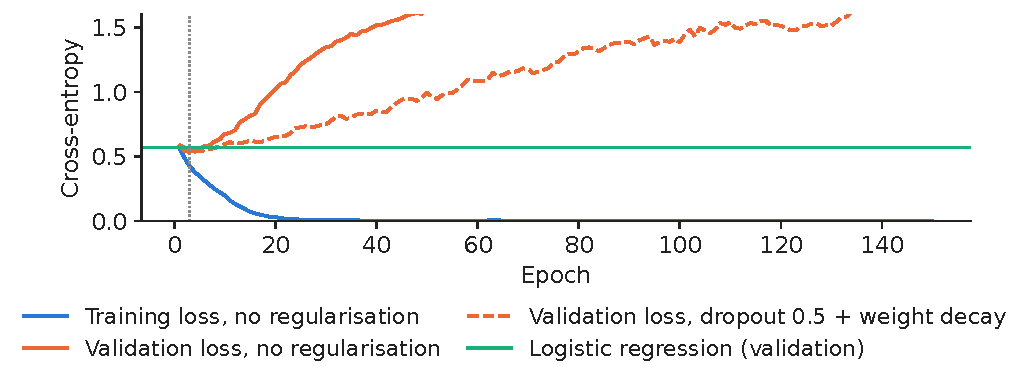
\includegraphics[width=\textwidth,height=0.394\textheight,keepaspectratio]{charts/en/overfit_german.pdf}\end{center}\vspace{-3mm}
\chartsource{Source: UCI Machine Learning Repository, Statlog German credit. Data: 600 training and 200 validation applicants; MLP 256-256.}
\vspace{0.5mm}
\begin{itemize}\setlength{\itemsep}{0pt}
  \item Validation loss 0.536 at epoch 3, 2.187 after 150
    \begin{itemize}\setlength{\itemsep}{0pt}
      \item With dropout and decay 1.767
      \item Logistic 0.570.
    \end{itemize}
\end{itemize}
\par\vfill\manager{a training loss near zero on credit data is a warning, not a success.}\par\vspace{0.5mm}
\par\vfill\noindent{\scriptsize\color{FooterGray}(own computation)}\hfill\qlink{NN\_L3\_overfit\_german}{Quantlets/L3/NN_L3_overfit_german}\par\vspace{0.5mm}
\end{frame}

\begin{frame}{The test error splits into bias, variance and noise}
\small
\intuition{a rigid model misses the pattern (bias), a flexible one chases the noise of its sample (variance).}
\[ \E_{\mathcal D,\varepsilon}\big[(y-\hat f_{\mathcal D}(x))^2\big]=\underbrace{\big(f(x)-\E_{\mathcal D}\hat f_{\mathcal D}(x)\big)^2}_{\text{bias}^2}+\underbrace{\Var_{\mathcal D}\big(\hat f_{\mathcal D}(x)\big)}_{\text{variance}}+\underbrace{\sigma^2}_{\text{noise}} \]
{\footnotesize\begin{itemize}\setlength{\itemsep}{0pt}
  \item \textbf{\txtwhere}
    \begin{itemize}\setlength{\itemsep}{0pt}
      \item $y=f(x)+\varepsilon$, $\Var(\varepsilon)=\sigma^2$, $\hat f_{\mathcal D}$ the model fitted on a random training sample $\mathcal D$, derivation in the appendix
    \end{itemize}
\end{itemize}\par}
\begin{itemize}\setlength{\itemsep}{2pt}
  \item Regularisation trades a little bias for a large cut in variance
    \begin{itemize}\setlength{\itemsep}{0pt}
      \item The noise $\sigma^2$ is a floor no model can beat.
    \end{itemize}
  \item Classical U-curve: test error first falls, then rises with capacity
    \begin{itemize}\setlength{\itemsep}{0pt}
      \item Very large networks can show a second descent (next frame).
    \end{itemize}
\end{itemize}
\par\vfill\manager{with few observations variance dominates: prefer simple models or strong regularisation.}\par\vspace{0.5mm}
\par\vfill\noindent{\scriptsize\color{FooterGray}(Hastie, Tibshirani \& Friedman, 2009, ch.~7)}\par\vspace{0.5mm}
\end{frame}

\begin{frame}{Past the interpolation threshold, more hidden units lower the test error again}
\small
\intuition{$p$ random, frozen rectified linear units (ReLU), minimum-norm output, $n=$ 400 block groups.}
\begin{center}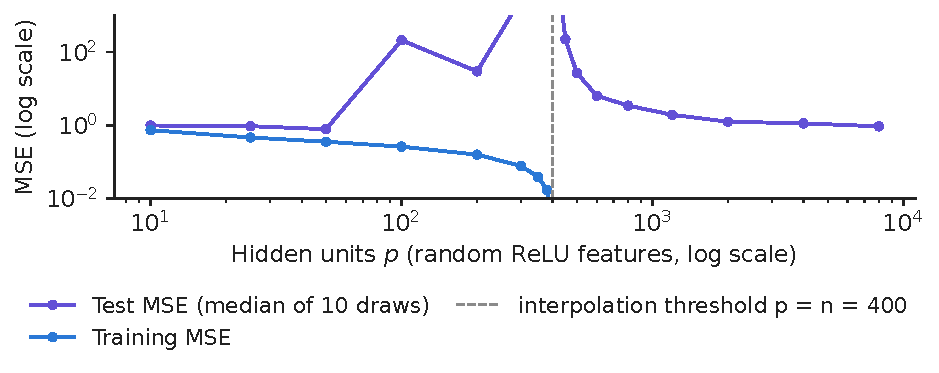
\includegraphics[width=\textwidth,height=0.348\textheight,keepaspectratio]{charts/en/double_descent.pdf}\end{center}\vspace{-3mm}
\chartsource{Source: StatLib, California housing, 1990 census (Pace and Barry, 1997). Data: 400 training and 5,000 test block groups per draw, 10 draws.}
\vspace{0.5mm}
\begin{itemize}\setlength{\itemsep}{0pt}
  \item Test mean squared error (MSE): 0.781 at $p=$ 50, $1.0\times10^{6}$ at $p=n$, 0.932 at $p=$ 8\,000 (median of 10 draws).
\end{itemize}
\par\vfill\manager{near $p=n$ a bigger model can be far worse, far past it size helps again.}\par\vspace{0.5mm}
\par\vfill\noindent{\scriptsize\color{FooterGray}(Belkin et al., 2019; Nakkiran et al., 2021)}\hfill\qlink{NN\_L3\_double\_descent}{Quantlets/L3/NN_L3_double_descent}\par\vspace{0.5mm}
\end{frame}


\section{Penalties on the weights}

\begin{frame}{Weight decay as an L2 penalty and as a Gaussian prior on the weights}
\small
\intuition{large weights make the function steep and sensitive to noise; shrinking them makes it smoother.}
\[ \tilde\loss(\vw)=\loss(\vw)+\frac\lambda2\|\vw\|_2^2\ \Rightarrow\ \vw_{t+1}=(1-\eta\lambda)\,\vw_t-\eta\nabla\loss(\vw_t);\qquad \vw\sim\mathcal N(\mathbf 0,\lambda^{-1}\mathbf I)\Rightarrow\hat\vw_{\mathrm{MAP}}=\argmin\tilde\loss \]
{\footnotesize\begin{itemize}\setlength{\itemsep}{0pt}
  \item \textbf{\txtwhere}
    \begin{itemize}\setlength{\itemsep}{0pt}
      \item $\lambda>0$ the penalty strength, $(1-\eta\lambda)$ the decay per stochastic gradient descent (SGD) step, maximum a posteriori (MAP) estimate
    \end{itemize}
\end{itemize}\par}
\begin{itemize}\setlength{\itemsep}{2pt}
  \item In a linear model this is ridge regression: along eigen-direction $k$, coefficients shrink by $\frac{d_k}{d_k+\lambda}$ (Hoerl \& Kennard, 1970).
  \item With Adam, an L2 term in the loss is rescaled per weight
    \begin{itemize}\setlength{\itemsep}{0pt}
      \item Adam with decoupled weight decay (AdamW) shrinks every weight by the same factor (Loshchilov \& Hutter, 2019).
    \end{itemize}
\end{itemize}
\par\vfill\manager{weight decay is the first regulariser to tune
    \begin{itemize}\setlength{\itemsep}{0pt}
      \item Search $\lambda$ on a log grid with validation.
    \end{itemize}}\par\vspace{0.5mm}
\par\vfill\noindent{\scriptsize\color{FooterGray}(Bishop \& Bishop, 2024, ch.~9)}\hfill\tryit{notebook \S3}\par\vspace{0.5mm}
\end{frame}

\begin{frame}{An L1 penalty sets weights exactly to zero}
\small
\intuition{the L1 ball has corners on the axes, so the penalised optimum often lands on one: sparsity.}
\[ \tilde\loss(\vw)=\loss(\vw)+\lambda\|\vw\|_1,\qquad \text{proximal step: }\ w_j\leftarrow\operatorname{sign}(u_j)\max\big(|u_j|-\eta\lambda,0\big),\ u_j=w_j-\eta\,\partial_j\loss \]
{\footnotesize\begin{itemize}\setlength{\itemsep}{0pt}
  \item \textbf{\txtwhere}
    \begin{itemize}\setlength{\itemsep}{0pt}
      \item $\|\vw\|_1=\sum_j|w_j|$, the soft-thresholding step sets small weights exactly to zero (the lasso of Tibshirani, 1996)
    \end{itemize}
\end{itemize}\par}
\begin{itemize}\setlength{\itemsep}{2pt}
  \item L1 on the first layer of an MLP acts as variable selection: an input whose outgoing weights are all zero is switched off.
  \item Elastic net mixes both: $\lambda_1\|\vw\|_1+\tfrac{\lambda_2}2\|\vw\|_2^2$.
\end{itemize}
\par\vfill\manager{use L1 when a short list of inputs is needed for the model documentation.}\par\vspace{0.5mm}
\par\vfill\noindent{\scriptsize\color{FooterGray}(Tibshirani, 1996)}\hfill\tryit{notebook \S3}\par\vspace{0.5mm}
\end{frame}

\begin{frame}{First-layer weights under L1 and L2 penalties}
\small
\intuition{MLP with 64 hidden units on German credit, full-batch Adam, penalty on the first layer only.}
\begin{center}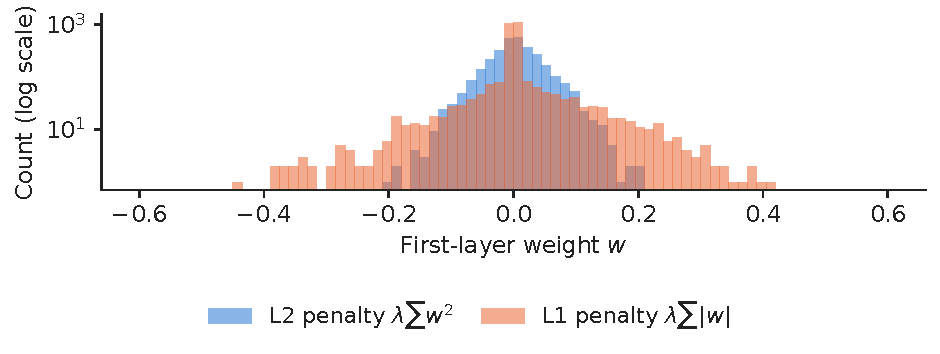
\includegraphics[width=\textwidth,height=0.397\textheight,keepaspectratio]{charts/en/l1_l2_weights.pdf}\end{center}\vspace{-3mm}
\chartsource{Source: UCI Machine Learning Repository, Statlog German credit. Data: 600 training applicants; MLP with 64 hidden units, 3,072 first-layer weights.}
\vspace{0.5mm}
\begin{itemize}\setlength{\itemsep}{0pt}
  \item Weights with $|w|<$ 0.01: 67.2\,\% under L1 against 26.3\,\% under L2 (3\,072 weights)
    \begin{itemize}\setlength{\itemsep}{0pt}
      \item Test AUC 0.768 with L1 against 0.761 with L2.
    \end{itemize}
\end{itemize}
\par\vfill\manager{a stronger L1 penalty would zero whole input columns, which can then leave the data pipeline.}\par\vspace{0.5mm}
\par\vfill\noindent{\scriptsize\color{FooterGray}(own computation)}\hfill\qlink{NN\_L3\_l1\_l2\_weights}{Quantlets/L3/NN_L3_l1_l2_weights}\par\vspace{0.5mm}
\end{frame}


\section{Dropout, early stopping and batch normalisation}

\begin{frame}{Dropout trains an ensemble of thinned networks that share their weights}
\small
\intuition{randomly silencing units forbids any unit to rely on a few others: features must be useful on their own.}
\[ \text{training: }\ \tilde h_j=\frac{m_j}{1-p}\,h_j,\ \ m_j\iid\text{Bernoulli}(1-p);\qquad \text{test: }\ \tilde h_j=h_j \]
{\footnotesize\begin{itemize}\setlength{\itemsep}{0pt}
  \item \textbf{\txtwhere}
    \begin{itemize}\setlength{\itemsep}{0pt}
      \item $p$ the dropout rate, $m_j$ the random mask, dividing by $1-p$ (inverted dropout) keeps $\E[\tilde h_j]=h_j$, so nothing changes at test time
    \end{itemize}
\end{itemize}\par}
\begin{itemize}\setlength{\itemsep}{2pt}
  \item A network with $H$ droppable units samples from $2^H$ sub-networks
    \begin{itemize}\setlength{\itemsep}{0pt}
      \item At test time the full network approximates their average (Srivastava et al., 2014).
    \end{itemize}
  \item Typical rates: 0.1--0.3 in a tabular MLP, 0.5 in large fully connected layers
    \begin{itemize}\setlength{\itemsep}{0pt}
      \item In PyTorch \texttt{model.eval()} switches it off.
    \end{itemize}
\end{itemize}
\par\vfill\manager{forgetting \texttt{model.eval()} before scoring makes every prediction random.}\par\vspace{0.5mm}
\par\vfill\noindent{\scriptsize\color{FooterGray}(Srivastava et al., 2014)}\hfill\tryit{notebook \S4}\par\vspace{0.5mm}
\end{frame}

\begin{frame}{On 600 applicants, regularisation does not close the gap to logistic regression}
\small
\intuition{MLP 256-256, 150 epochs without early stopping; held-out AUC over 5 folds for each $\lambda$ and $p$.}
\begin{center}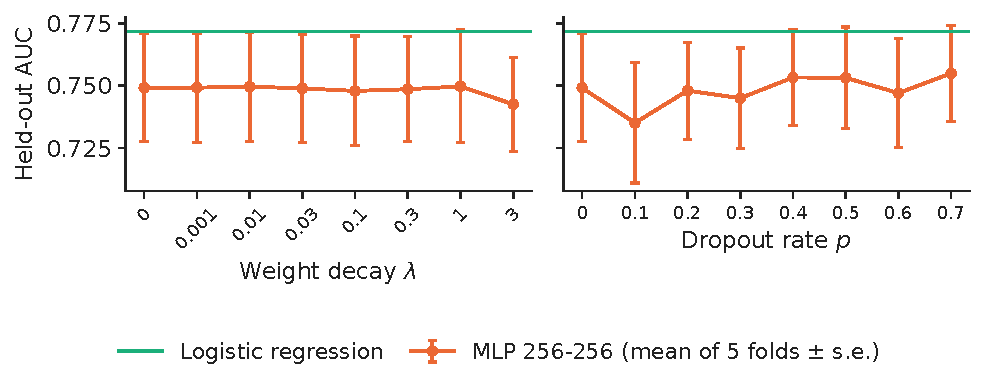
\includegraphics[width=\textwidth,height=0.329\textheight,keepaspectratio]{charts/en/wd_dropout.pdf}\end{center}\vspace{-3mm}
\chartsource{Source: UCI Machine Learning Repository, Statlog German credit. Data: 1,000 applicants, 5-fold cross-validation, no early stopping (150 epochs).}
\vspace{0.5mm}
\begin{itemize}\setlength{\itemsep}{0pt}
  \item AUC 0.749 unregularised, 0.750 at $\lambda=$ 1, 0.755 at $p=$ 0.7
    \begin{itemize}\setlength{\itemsep}{0pt}
      \item Logistic 0.772
      \item Weight norm 18.0 vs 10.6 at $\lambda=3$.
    \end{itemize}
\end{itemize}
\par\vfill\manager{on very small data, a smaller model beats a large regularised one.}\par\vspace{0.5mm}
\par\vfill\noindent{\scriptsize\color{FooterGray}(own computation)}\hfill\qlink{NN\_L3\_wd\_dropout}{Quantlets/L3/NN_L3_wd_dropout}\par\vspace{0.5mm}
\end{frame}

\begin{frame}{Early stopping: keep the weights of the best validation epoch}
\small
\intuition{training longer fits more noise; stop when the validation loss has not improved for a while.}
\[ t^*=\argmin_{t\le T}\ \loss_{\text{val}}(\vw_t),\quad \text{stop when}\ t-t^*\ge P;\qquad \text{quadratic loss:}\ \ \eta\,t\ \approx\ \frac1\lambda \]
{\footnotesize\begin{itemize}\setlength{\itemsep}{0pt}
  \item \textbf{\txtwhere}
    \begin{itemize}\setlength{\itemsep}{0pt}
      \item $P$ the patience in epochs, the last relation says that $t$ steps of size $\eta$ act like an L2 penalty of strength $\lambda\approx1/(\eta t)$ (appendix)
    \end{itemize}
\end{itemize}\par}
\begin{itemize}\setlength{\itemsep}{2pt}
  \item The validation set is used for the stopping decision: it is no longer an unbiased estimate, so a separate test set is needed.
  \item Free, cheap and compatible with every other regulariser (Prechelt, 1998).
\end{itemize}
\par\vfill\manager{save the best checkpoint, not the last one.}\par\vspace{0.5mm}
\par\vfill\noindent{\scriptsize\color{FooterGray}(Prechelt, 1998; Bishop \& Bishop, 2024, ch.~9)}\hfill\tryit{notebook \S5}\par\vspace{0.5mm}
\end{frame}

\begin{frame}{On card fraud, validation loss bottoms out early while training loss keeps falling}
\small
\intuition{MLP 256-256, time-ordered split; dashed: best validation epoch; grey: the patience window.}
\begin{center}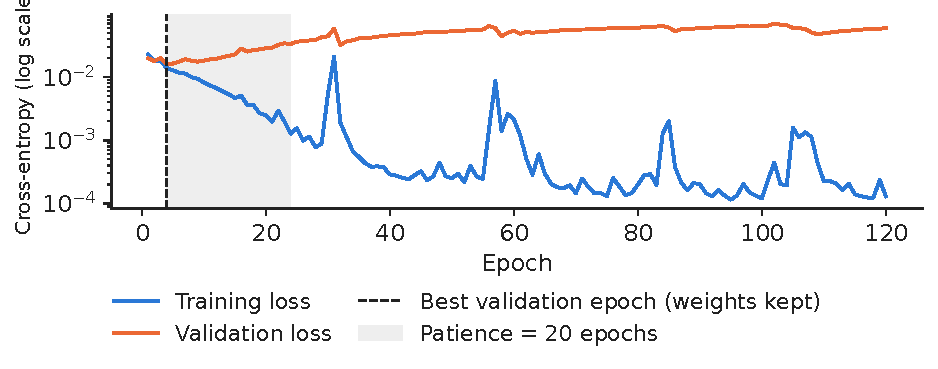
\includegraphics[width=\textwidth,height=0.408\textheight,keepaspectratio]{charts/en/early_stopping.pdf}\end{center}\vspace{-3mm}
\chartsource{Source: ULB Machine Learning Group and Worldline, credit-card transactions (OpenML 1597). Data: time-ordered split: 17,354 training, 5,785 validation transactions.}
\vspace{0.5mm}
\begin{itemize}\setlength{\itemsep}{0pt}
  \item Best epoch 4, stop at 24 (patience 20)
    \begin{itemize}\setlength{\itemsep}{0pt}
      \item Validation loss 0.0159 there, 0.0593 after 120 epochs.
    \end{itemize}
\end{itemize}
\par\vfill\manager{with rare events the network starts memorising the few training frauds within a handful of epochs.}\par\vspace{0.5mm}
\par\vfill\noindent{\scriptsize\color{FooterGray}(own computation)}\hfill\qlink{NN\_L3\_early\_stopping}{Quantlets/L3/NN_L3_early_stopping}\par\vspace{0.5mm}
\end{frame}

\begin{frame}{Batch normalisation standardises each unit over the mini-batch}
\small
\intuition{keeping pre-activations centred and scaled lets deep networks train with larger steps.}
\[ \hat z_{ij}=\frac{z_{ij}-\mu_{\mathcal B,j}}{\sqrt{\sigma^2_{\mathcal B,j}+\epsilon}},\qquad y_{ij}=\gamma_j\hat z_{ij}+\beta_j,\qquad \mu_{\mathcal B,j}=\frac1B\sum_{i\in\mathcal B}z_{ij} \]
{\footnotesize\begin{itemize}\setlength{\itemsep}{0pt}
  \item \textbf{\txtwhere}
    \begin{itemize}\setlength{\itemsep}{0pt}
      \item $\sigma^2_{\mathcal B,j}$ the batch variance of unit $j$, $\gamma_j,\beta_j$ learned scale and shift, at test time running averages replace the batch statistics
    \end{itemize}
\end{itemize}\par}
\begin{itemize}\setlength{\itemsep}{2pt}
  \item Batch normalisation (BN) smooths the loss landscape, which tolerates larger learning rates (Ioffe \& Szegedy, 2015).
  \item The batch statistics add noise to each example's output: a mild regulariser
    \begin{itemize}\setlength{\itemsep}{0pt}
      \item Layer normalisation (Lecture 7) avoids the batch dependence.
    \end{itemize}
\end{itemize}
\par\vfill\manager{with batch norm, \texttt{model.eval()} is mandatory and very small batches should be avoided.}\par\vspace{0.5mm}
\par\vfill\noindent{\scriptsize\color{FooterGray}(Ioffe \& Szegedy, 2015)}\hfill\tryit{notebook \S6}\par\vspace{0.5mm}
\end{frame}

\begin{frame}{Batch norm lets a deep MLP train at a rate at which it otherwise diverges}
\small
\intuition{6 hidden layers of 64 units on California housing, SGD with momentum; medians of 3 seeds.}
\begin{center}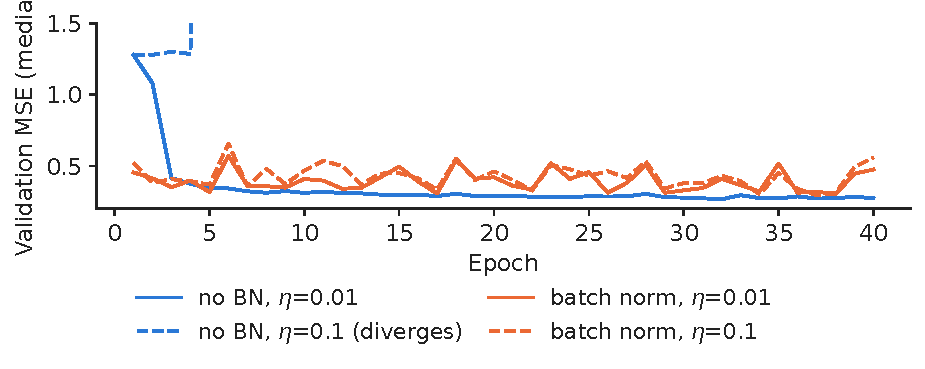
\includegraphics[width=\textwidth,height=0.321\textheight,keepaspectratio]{charts/en/batchnorm.pdf}\end{center}\vspace{-3mm}
\chartsource{Source: StatLib, California housing, 1990 census (Pace and Barry, 1997). Data: 6 hidden layers of 64 units, SGD with momentum 0.9, 3 seeds.}
\vspace{0.5mm}
\begin{itemize}\setlength{\itemsep}{0pt}
  \item At $\eta=0.1$: 3 of 3 seeds diverge without BN, best validation MSE 0.283 with BN
    \begin{itemize}\setlength{\itemsep}{0pt}
      \item At $\eta=0.01$: 0.265 without, 0.277 with BN.
    \end{itemize}
\end{itemize}
\par\vfill\manager{batch norm is mainly an optimisation aid
    \begin{itemize}\setlength{\itemsep}{0pt}
      \item Keep early stopping, its validation error fluctuates.
    \end{itemize}}\par\vspace{0.5mm}
\par\vfill\noindent{\scriptsize\color{FooterGray}(own computation)}\hfill\qlink{NN\_L3\_batchnorm}{Quantlets/L3/NN_L3_batchnorm}\par\vspace{0.5mm}
\end{frame}

\begin{frame}{Other regularisers: more data, noise, ensembles}
\small
\begin{columns}[T,onlytextwidth]
\begin{column}{0.50\textwidth}
\begin{itemize}\setlength{\itemsep}{2pt}
  \item \textbf{Data augmentation}: label-preserving transformations (crops and flips for images, Lecture 4)
    \begin{itemize}\setlength{\itemsep}{0pt}
      \item For tabular data, rarely safe.
    \end{itemize}
  \item \textbf{Noise injection}: Gaussian noise on the inputs is equivalent, to first order, to an L2 penalty on the input gradient.
  \item \textbf{Label smoothing}: train on $(1-\epsilon)y+\epsilon/2$ instead of 0/1 targets
    \begin{itemize}\setlength{\itemsep}{0pt}
      \item Curbs over-confident probabilities.
    \end{itemize}
\end{itemize}
\end{column}
\begin{column}{0.47\textwidth}
\begin{itemize}\setlength{\itemsep}{2pt}
  \item \textbf{Ensembles}: average several seeds or models
    \begin{itemize}\setlength{\itemsep}{0pt}
      \item Variance falls roughly as $1/M$ for $M$ weakly correlated members.
    \end{itemize}
  \item \textbf{Smaller model or fewer inputs}: the oldest regulariser.
  \item \textbf{More data}: the only one with no side effects
    \begin{itemize}\setlength{\itemsep}{0pt}
      \item One more year of transactions beats any penalty.
    \end{itemize}
\end{itemize}
\end{column}
\end{columns}
\par\vfill\manager{our fraud case averages 5 seeds: a cheap ensemble that also reports the uncertainty.}\par\vspace{0.5mm}
\par\vfill\noindent{\scriptsize\color{FooterGray}(Bishop \& Bishop, 2024, ch.~9)}\par\vspace{0.5mm}
\end{frame}


\section{Validation design}

\begin{frame}{Hold-out, cross-validation and nested cross-validation}
\small
\intuition{every choice made by looking at data must be paid for with data the choice has not seen.}
\[ \widehat{\mathrm{CV}}_K=\frac1K\sum_{k=1}^{K}\frac1{|\mathcal D_k|}\sum_{i\in\mathcal D_k}\ell\big(y_i,\hat f^{(-k)}(\vx_i)\big) \]
{\footnotesize\begin{itemize}\setlength{\itemsep}{0pt}
  \item \textbf{\txtwhere}
    \begin{itemize}\setlength{\itemsep}{0pt}
      \item $\mathcal D_k$ fold $k$, $\hat f^{(-k)}$ the model fitted on the other $K-1$ folds, usually $K=5$ or 10, stratified on the label
    \end{itemize}
\end{itemize}\par}
\begin{itemize}\setlength{\itemsep}{2pt}
  \item Hold-out: one train/validation/test split
    \begin{itemize}\setlength{\itemsep}{0pt}
      \item Cheap, but noisy on small data (next frame).
    \end{itemize}
  \item Nested cross-validation: an inner loop tunes hyperparameters, an outer loop measures the whole tuning procedure.
  \item Report the spread across folds, not only the mean
    \begin{itemize}\setlength{\itemsep}{0pt}
      \item Compare models with the corrected $t$-test of Lecture 1.
    \end{itemize}
\end{itemize}
\par\vfill\manager{the reported performance must come from data used neither for fitting nor for choosing.}\par\vspace{0.5mm}
\par\vfill\noindent{\scriptsize\color{FooterGray}(Hastie, Tibshirani \& Friedman, 2009, ch.~7)}\hfill\tryit{notebook \S7}\par\vspace{0.5mm}
\end{frame}

\begin{frame}{One random hold-out split can move the AUC by several points}
\small
\intuition{logistic regression on German credit, 200 random stratified 70/30 splits of the same applicants.}
\begin{center}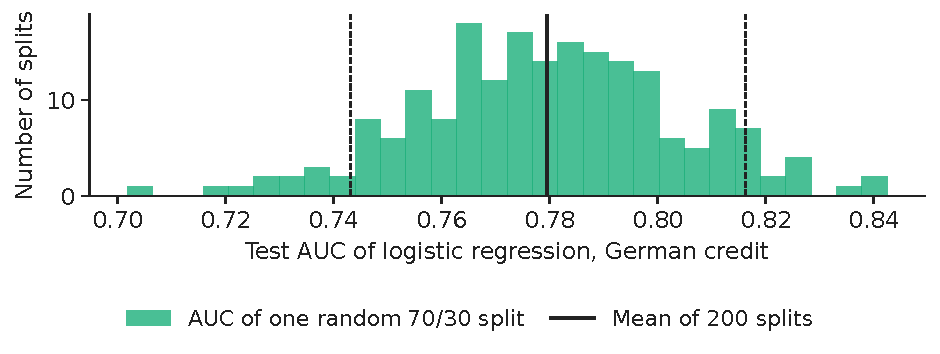
\includegraphics[width=\textwidth,height=0.433\textheight,keepaspectratio]{charts/en/holdout_noise.pdf}\end{center}\vspace{-3mm}
\chartsource{Source: UCI Machine Learning Repository, Statlog German credit. Data: 1,000 applicants, 200 random stratified splits.}
\vspace{0.5mm}
\begin{itemize}\setlength{\itemsep}{0pt}
  \item Test AUC from 0.702 to 0.842
    \begin{itemize}\setlength{\itemsep}{0pt}
      \item 90\,\% of splits in [0.743; 0.816], standard deviation 0.024.
    \end{itemize}
\end{itemize}
\par\vfill\manager{on a small dataset, one split cannot separate two models: use repeated cross-validation.}\par\vspace{0.5mm}
\par\vfill\noindent{\scriptsize\color{FooterGray}(own computation)}\hfill\qlink{NN\_L3\_holdout\_noise}{Quantlets/L3/NN_L3_holdout_noise}\par\vspace{0.5mm}
\end{frame}

\begin{frame}{Information leakage into the validation set}
\small
\intuition{any information from the evaluation rows that reaches training inflates the score and disappears in production.}
{\scriptsize\renewcommand{\arraystretch}{1.05}\setlength{\tabcolsep}{4pt}
\begin{tabular}{@{}p{0.27\textwidth}p{0.36\textwidth}p{0.30\textwidth}@{}}\toprule
Leak & Example & Fix \\ \midrule
Preprocessing on all rows & scaler or imputer fitted before the split & fit on the training part only \\
Resampling before the split & copies of a fraud in both train and test & oversample inside the training fold \\
Ignoring time & random split of a time series or of payments & train on the past, test on the future \\
Target in the inputs & `days past due' used to predict default & keep only information known at decision time \\
\bottomrule\end{tabular}}
\par\vspace{0.5mm}{\scriptsize \begin{itemize}\setlength{\itemsep}{0pt}
  \item Time series: expanding-window or blocked cross-validation; never shuffle (Bergmeir \& Benítez, 2012).
\end{itemize}}
\par\vfill\manager{write down, for every input, the moment it becomes known.}\par\vspace{0.5mm}
\par\vfill\noindent{\scriptsize\color{FooterGray}(Kaufman et al., 2012)}\hfill\tryit{notebook \S8}\par\vspace{0.5mm}
\end{frame}

\begin{frame}{Oversampling before the split overstates performance}
\small
\intuition{the same MLP 128-128 and the same transactions, evaluated three ways; 5 seeds each.}
\begin{center}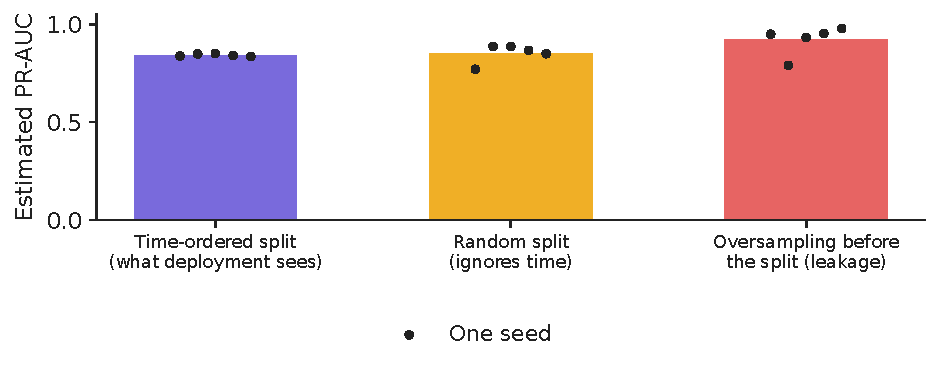
\includegraphics[width=\textwidth,height=0.388\textheight,keepaspectratio]{charts/en/split_leakage.pdf}\end{center}\vspace{-3mm}
\chartsource{Source: ULB Machine Learning Group and Worldline, credit-card transactions (OpenML 1597). Data: the same 28,924 transactions, MLP 128-128 with early stopping, 5 seeds.}
\vspace{0.5mm}
\begin{itemize}\setlength{\itemsep}{0pt}
  \item PR-AUC 0.843 with a time-ordered split, 0.853 with a random split, 0.921 with frauds copied 20 times before splitting.
\end{itemize}
\par\vfill\manager{only the time-ordered estimate describes what the bank will see after deployment.}\par\vspace{0.5mm}
\par\vfill\noindent{\scriptsize\color{FooterGray}(own computation)}\hfill\qlink{NN\_L3\_split\_leakage}{Quantlets/L3/NN_L3_split_leakage}\par\vspace{0.5mm}
\end{frame}


\section{Case study: card fraud detection}

\begin{frame}{Fraud is rare and clustered in time}
\small
\intuition{Université libre de Bruxelles (ULB) and Worldline data, Open Machine Learning platform (OpenML): two days of card payments.}
\begin{center}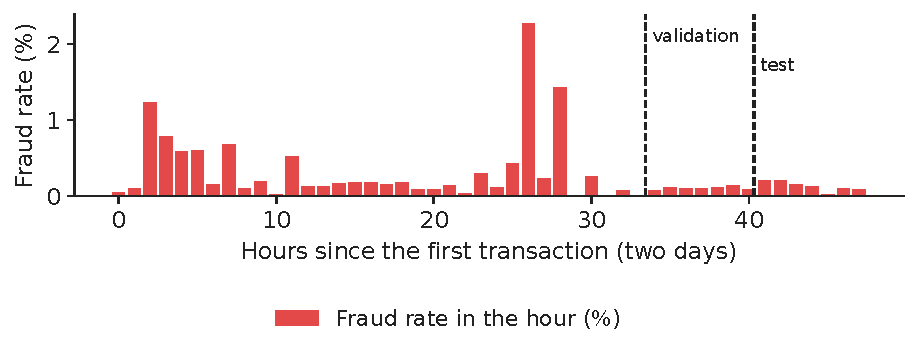
\includegraphics[width=\textwidth,height=0.325\textheight,keepaspectratio]{charts/en/fraud_by_hour.pdf}\end{center}\vspace{-3mm}
\chartsource{Source: ULB Machine Learning Group and Worldline, credit-card transactions (OpenML 1597). Data: September 2013, 2 days, 284,807 transactions (weighted sample).}
\vspace{0.5mm}
\begin{itemize}\setlength{\itemsep}{0pt}
  \item 284\,807 payments, fraud rate 0.173\,\%
    \begin{itemize}\setlength{\itemsep}{0pt}
      \item We keep all 492 frauds and 10\,\% of legitimate payments (weight 10)
      \item Inputs: 28 principal component analysis (PCA) scores and the log amount.
    \end{itemize}
\end{itemize}
\par\vfill\manager{the hourly rate swings strongly: a random split would mix calm and attack hours.}\par\vspace{0.5mm}
\par\vfill\noindent{\scriptsize\color{FooterGray}(Dal Pozzolo et al., 2015)}\hfill\qlink{NN\_L3\_fraud\_by\_hour}{Quantlets/L3/NN_L3_fraud_by_hour}\par\vspace{0.5mm}
\end{frame}

\begin{frame}{Performance measures for rare events: precision, recall and PR-AUC}
\small
\intuition{flagging nothing is 99.8\,\% accurate; the bank cares how many alerts are frauds and how many frauds raise an alert.}
\[ \text{precision}=\frac{TP}{TP+FP},\quad \text{recall}=\frac{TP}{TP+FN},\quad \text{PR-AUC}=\sum_k(R_k-R_{k-1})\,P_k \]
{\footnotesize\begin{itemize}\setlength{\itemsep}{0pt}
  \item \textbf{\txtwhere}
    \begin{itemize}\setlength{\itemsep}{0pt}
      \item $TP$, $FP$, $FN$ true positives, false positives, false negatives at a cut-off, $P_k,R_k$ precision and recall at the $k$-th threshold
    \end{itemize}
\end{itemize}\par}
\begin{itemize}\setlength{\itemsep}{2pt}
  \item PR-AUC depends on the fraud rate (a random score gets PR-AUC = fraud rate)
    \begin{itemize}\setlength{\itemsep}{0pt}
      \item AUC does not, which hides the false alarms (Saito \& Rehmsmeier, 2015).
    \end{itemize}
  \item Undersampled data: every legitimate payment counts with weight 10.00 in $FP$, so precision is that of the full population.
\end{itemize}
\par\vfill\manager{report precision at the recall the investigation team can handle.}\par\vspace{0.5mm}
\par\vfill\noindent{\scriptsize\color{FooterGray}(Saito \& Rehmsmeier, 2015)}\hfill\tryit{notebook \S9}\par\vspace{0.5mm}
\end{frame}

\begin{frame}{On the test hours, early stopping is the regulariser with the clearest gain}
\small
\intuition{MLP 256-256, time-ordered split, 5 seeds per configuration; precision weighted to the population.}
\begin{center}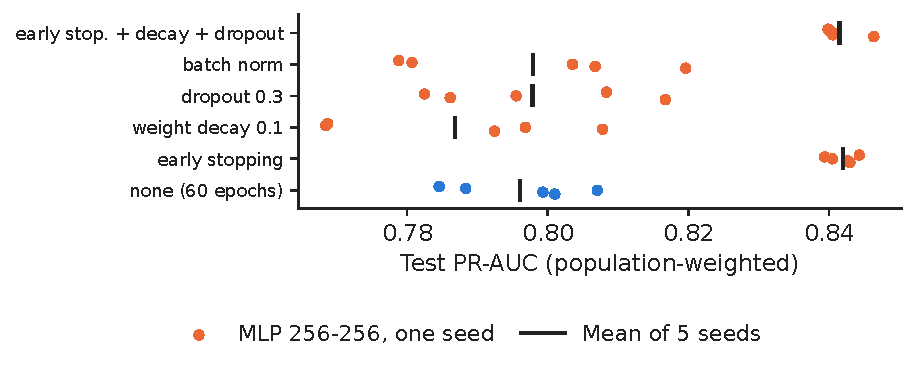
\includegraphics[width=\textwidth,height=0.388\textheight,keepaspectratio]{charts/en/reg_ablation.pdf}\end{center}\vspace{-3mm}
\chartsource{Source: ULB Machine Learning Group and Worldline, credit-card transactions (OpenML 1597). Data: time-ordered test set: last 5,785 transactions (75 frauds); 5 seeds.}
\vspace{0.5mm}
\begin{itemize}\setlength{\itemsep}{0pt}
  \item Test PR-AUC: none 0.796, early stopping 0.842, decay 0.787, dropout 0.798, batch norm 0.798, all 0.841.
\end{itemize}
\par\vfill\manager{with 60 fixed epochs, the other regularisers stay within the seed noise.}\par\vspace{0.5mm}
\par\vfill\noindent{\scriptsize\color{FooterGray}(own computation)}\hfill\qlink{NN\_L3\_reg\_ablation}{Quantlets/L3/NN_L3_reg_ablation}\par\vspace{0.5mm}
\end{frame}

\begin{frame}{The regularised MLP compared with logistic regression and gradient boosting}
\small
\intuition{test hours (last 20\,\%); the MLP averages 5 seeds with early stopping, decay and dropout.}
\begin{center}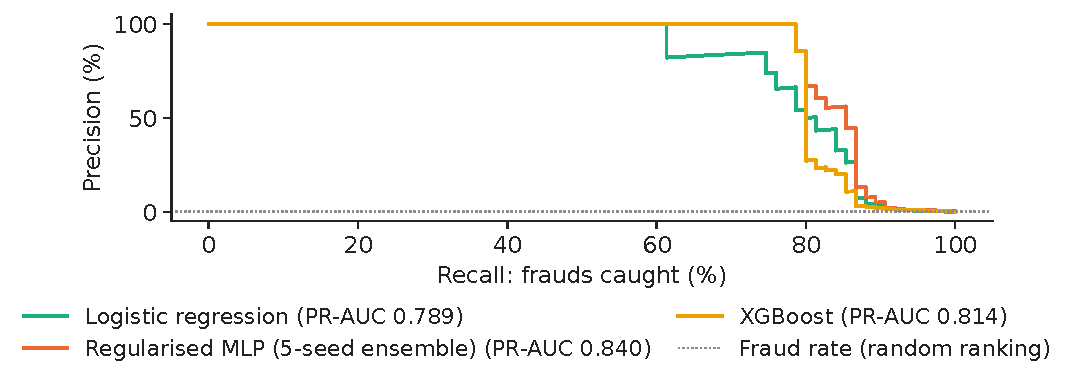
\includegraphics[width=\textwidth,height=0.401\textheight,keepaspectratio]{charts/en/fraud_pr.pdf}\end{center}\vspace{-3mm}
\chartsource{Source: ULB Machine Learning Group and Worldline, credit-card transactions (OpenML 1597). Data: time-ordered test set: 5,785 transactions, 75 frauds, population-weighted.}
\vspace{0.5mm}
\begin{itemize}\setlength{\itemsep}{0pt}
  \item PR-AUC: logistic 0.789, MLP 0.840, extreme gradient boosting (XGBoost) 0.814
    \begin{itemize}\setlength{\itemsep}{0pt}
      \item Recall at 80\,\% precision 74.7, 80.0, 80.0\,\%.
    \end{itemize}
\end{itemize}
\par\vfill\manager{with 75 test frauds, a few points of difference are within the noise.}\par\vspace{0.5mm}
\par\vfill\noindent{\scriptsize\color{FooterGray}(own computation)}\hfill\qlink{NN\_L3\_fraud\_pr}{Quantlets/L3/NN_L3_fraud_pr}\par\vspace{0.5mm}
\end{frame}

\begin{frame}{Class weights and the prior correction for undersampled data}
\small
\intuition{weighting the rare class changes the scores' level, not only their order; after undersampling, probabilities must be corrected.}
\[ \loss_w=-\frac1n\sum_i\big[w_+\,y_i\log p_i+w_-\,(1-y_i)\log(1-p_i)\big],\qquad p=\frac{\beta\,p_s}{\beta\,p_s-p_s+1} \]
{\footnotesize\begin{itemize}\setlength{\itemsep}{0pt}
  \item \textbf{\txtwhere}
    \begin{itemize}\setlength{\itemsep}{0pt}
      \item $w_\pm$ class weights, $p_s$ the probability learned on data where legitimate payments were kept with rate $\beta$ (here 0.1), $p$ the corrected probability
    \end{itemize}
\end{itemize}\par}
\begin{itemize}\setlength{\itemsep}{2pt}
  \item Class weights or resampling change the effective cut-off
    \begin{itemize}\setlength{\itemsep}{0pt}
      \item The ranking, and thus PR-AUC, changes little.
    \end{itemize}
  \item Whatever is done, the cut-off should come from costs (next frame), and probabilities must be corrected before they are used as such.
\end{itemize}
\par\vfill\manager{never report probabilities from a resampled model to the business without the prior correction.}\par\vspace{0.5mm}
\par\vfill\noindent{\scriptsize\color{FooterGray}(Dal Pozzolo et al., 2015)}\hfill\tryit{notebook \S10}\par\vspace{0.5mm}
\end{frame}

\begin{frame}{Number of alerts and the share of fraud losses avoided}
\small
\intuition{a missed fraud costs its amount; each alert costs a review of 5 euro (EUR), a constant chosen a priori.}
\begin{center}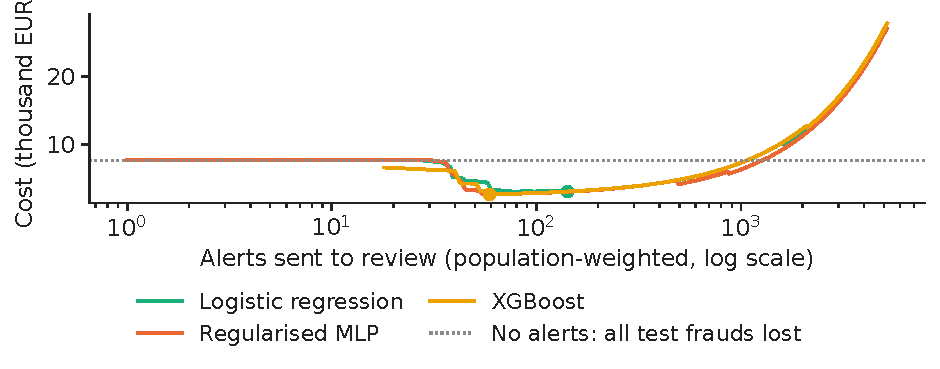
\includegraphics[width=\textwidth,height=0.401\textheight,keepaspectratio]{charts/en/fraud_cost.pdf}\end{center}\vspace{-3mm}
\chartsource{Source: ULB Machine Learning Group and Worldline, credit-card transactions (OpenML 1597). Data: test period (last 20\,\% of the two days); review cost 5 EUR per alert.}
\vspace{0.5mm}
\begin{itemize}\setlength{\itemsep}{0pt}
  \item Test losses with no alerts 7\,729 EUR
    \begin{itemize}\setlength{\itemsep}{0pt}
      \item At the best alert count: logistic 3\,093, MLP 2\,694, XGBoost 2\,695 EUR.
    \end{itemize}
\end{itemize}
\par\vfill\manager{the alert budget is the business decision, the model only ranks.}\par\vspace{0.5mm}
\par\vfill\noindent{\scriptsize\color{FooterGray}(own computation)}\hfill\qlink{NN\_L3\_fraud\_cost}{Quantlets/L3/NN_L3_fraud_cost}\par\vspace{0.5mm}
\end{frame}

\begin{frame}{Summary of regularisation methods}
\small
{\scriptsize\renewcommand{\arraystretch}{1.05}\setlength{\tabcolsep}{4pt}
\begin{tabular}{@{}p{0.17\textwidth}p{0.30\textwidth}p{0.22\textwidth}p{0.25\textwidth}@{}}\toprule
Method & What it does & Main knob & On our data \\ \midrule
Weight decay & shrinks all weights & $\lambda$ & smaller weights, same AUC (German) \\
L1 & sets weights to zero & $\lambda$ & most first-layer weights near zero \\
Dropout & trains an ensemble of sub-networks & $p$ & within seed noise \\
Early stopping & stops before memorising & patience $P$ & clear gain on fraud \\
Batch norm & stabilises training & batch size & trains at $\eta$ where plain SGD diverges \\
Smaller model & fewer parameters & width, depth & logistic beats MLP on German credit \\
\bottomrule\end{tabular}}
\par\vfill\manager{start with early stopping and a modest model, then tune weight decay
    \begin{itemize}\setlength{\itemsep}{0pt}
      \item Add dropout and batch norm for deep networks.
    \end{itemize}}\par\vspace{0.5mm}
\end{frame}


\section{Wrap-up}

\begin{frame}{Key takeaways}
\small
\begin{itemize}\setlength{\itemsep}{4pt}
  \item Overfitting shows as a falling training loss with a rising validation loss
    \begin{itemize}\setlength{\itemsep}{0pt}
      \item On small data it starts within a few epochs.
    \end{itemize}
  \item Weight decay (Gaussian prior), L1 (sparsity), dropout (ensemble), early stopping (implicit L2) and batch norm (optimisation aid) control capacity in different ways.
  \item Very large models can show double descent: the classical U-curve is not the whole story.
  \item Validation must mimic deployment: time-ordered splits, preprocessing and resampling inside the training part only (PR-AUC 0.843 honest vs 0.921 leaked).
  \item For rare events, use PR-AUC, precision at a workable recall and the cost of errors, with several seeds.
\end{itemize}
\end{frame}

\begin{frame}{Key equations}
\small
\begin{columns}[T,onlytextwidth]
\begin{column}{0.49\textwidth}
\[ \E(y-\hat f)^2=\text{bias}^2+\Var(\hat f)+\sigma^2 \]
\[ \vw_{t+1}=(1-\eta\lambda)\vw_t-\eta\nabla\loss \]
\[ w_j\leftarrow\operatorname{sign}(u_j)(|u_j|-\eta\lambda)_+ \]
\[ \tilde h_j=m_jh_j/(1-p) \]
\end{column}
\begin{column}{0.49\textwidth}
\[ \hat z=(z-\mu_{\mathcal B})/\sqrt{\sigma^2_{\mathcal B}+\epsilon} \]
\[ \eta\,t^*\approx1/\lambda \]
\[ P=\tfrac{TP}{TP+FP},\ R=\tfrac{TP}{TP+FN} \]
\[ p=\beta p_s/(\beta p_s-p_s+1) \]
\end{column}
\end{columns}
\end{frame}

\begin{frame}{Research from our group: fraud detection and early warning}
\small
\begin{itemize}\setlength{\itemsep}{5pt}
  \item \textbf{Explainable artificial intelligence (AI) for fraud} (Diaconu \& Pele, 2026): on the Institute of Electrical and Electronics Engineers, Computational Intelligence Society (IEEE-CIS) fraud data, XGBoost and CatBoost had the higher AUC, while a graph neural network (GNN), graph sample and aggregate (GraphSAGE), captured relational fraud patterns that tabular models cannot describe.
  \item \textbf{Explaining at several levels}: their explainable AI (XAI) framework combines Shapley additive explanations (SHAP) for variables with node and edge ablation for the graph
    \begin{itemize}\setlength{\itemsep}{0pt}
      \item The paper concludes that fraud explanations should combine several model types --- replicated in Case study 1 (course site).
    \end{itemize}
  \item \textbf{Early warning of crypto `zombies'} (Będowska-Sójka, Wójcik \& Pele, 2026): machine-learning early warning systems that predict which crypto-assets become `zombie' assets
    \begin{itemize}\setlength{\itemsep}{0pt}
      \item An early-warning model must be validated forward in time, as in Section 4.
    \end{itemize}
\end{itemize}
\par\vspace{0.5mm}{\scriptsize \begin{itemize}\setlength{\itemsep}{0pt}
  \item Findings as stated in the papers; numbers on the other slides come from our own computations.
\end{itemize}}
\end{frame}

\begin{frame}{Further reading and resources}
\small
\begin{columns}[T,onlytextwidth]
\begin{column}{0.52\textwidth}
\begin{itemize}\setlength{\itemsep}{4pt}
  \item \textbf{Bishop \& Bishop (2024)}, chapter 9: regularisation: \href{https://www.bishopbook.com}{bishopbook.com}.
  \item \textbf{Hastie, Tibshirani \& Friedman (2009)}, chapter 7: model assessment and selection: \href{https://hastie.su.domains/ElemStatLearn/}{hastie.su.domains}.
  \item \textbf{Dive into Deep Learning}, sections 3.7, 5.6, 8.5: \href{https://d2l.ai}{d2l.ai}.
\end{itemize}
\end{column}
\begin{column}{0.45\textwidth}
\begin{itemize}\setlength{\itemsep}{4pt}
  \item \textbf{Fraud detection handbook} (Le Borgne et al., ULB): \href{https://fraud-detection-handbook.github.io/fraud-detection-handbook/}{fraud-detection-handbook.github.io}.
  \item \textbf{This course}: code, data, notebooks, Quantlets --- \href{https://github.com/danpele/NEURAL_BIZ}{github.com/danpele/NEURAL\_BIZ}.
  \item \textbf{Leakage}: Kaufman et al.\ (2012).
\end{itemize}
\end{column}
\end{columns}
\end{frame}

\begin{frame}{Quiz 1: reading the curves}
\small
\begin{itemize}
  \item Training loss keeps falling, validation loss rises after epoch 3.
    \begin{itemize}\setlength{\itemsep}{0pt}
      \item What do you do?
    \end{itemize}
\end{itemize}
\vspace{2mm}
\begin{exampleblock}{Answer}
\begin{itemize}
  \item The network overfits: keep the weights of epoch 3 (early stopping) and add weight decay or dropout
    \begin{itemize}\setlength{\itemsep}{0pt}
      \item Do not train longer.
    \end{itemize}
\end{itemize}
\end{exampleblock}
\end{frame}

\begin{frame}{Quiz 2: L1 or L2}
\small
\begin{itemize}
  \item Which penalty can switch an input off completely, and why?
\end{itemize}
\vspace{2mm}
\begin{exampleblock}{Answer}
\begin{itemize}
  \item L1: its soft-thresholding step sets small weights exactly to zero
    \begin{itemize}\setlength{\itemsep}{0pt}
      \item Here 67.2\,\% of the first-layer weights are below 0.01 (L2: 26.3\,\%).
    \end{itemize}
\end{itemize}
\end{exampleblock}
\end{frame}

\begin{frame}{Quiz 3: dropout at test time}
\small
\begin{itemize}
  \item With inverted dropout and $p=0.3$, what must be done to the activations at test time?
\end{itemize}
\vspace{2mm}
\begin{exampleblock}{Answer}
\begin{itemize}
  \item Nothing: dividing by $1-p$ during training already keeps the expectation
    \begin{itemize}\setlength{\itemsep}{0pt}
      \item Just call \texttt{model.eval()}.
    \end{itemize}
\end{itemize}
\end{exampleblock}
\end{frame}

\begin{frame}{Quiz 4: oversampling}
\small
\begin{itemize}
  \item Why does oversampling frauds before the split raise PR-AUC from 0.843 to 0.921?
\end{itemize}
\vspace{2mm}
\begin{exampleblock}{Answer}
\begin{itemize}
  \item Copies of the same fraud land in training and test, so the model is tested on frauds it has memorised
    \begin{itemize}\setlength{\itemsep}{0pt}
      \item Part of the gap is also the ignored time order.
    \end{itemize}
\end{itemize}
\end{exampleblock}
\end{frame}

\begin{frame}{Quiz 5: the right metric}
\small
\begin{itemize}
  \item A fraud model has AUC 0.977.
    \begin{itemize}\setlength{\itemsep}{0pt}
      \item Is that enough to deploy it?
    \end{itemize}
\end{itemize}
\vspace{2mm}
\begin{exampleblock}{Answer}
\begin{itemize}
  \item No: with a fraud rate of 0.173\,\% a high AUC can hide many false alarms
    \begin{itemize}\setlength{\itemsep}{0pt}
      \item Check PR-AUC (0.840), precision at the target recall and the cost of alerts.
    \end{itemize}
\end{itemize}
\end{exampleblock}
\end{frame}

\begin{frame}{References (1/2)}
\scriptsize
\begin{itemize}\setlength{\itemsep}{0pt}\scriptsize
\item Będowska-Sójka, B., Wójcik, P.\ \& Pele, D.\,T.\ (2026). Early warning systems for cryptocurrency markets: Predicting `zombie' assets using machine learning. \textit{The North American Journal of Economics and Finance}, 81, 102543. \href{https://doi.org/10.1016/j.najef.2025.102543}{doi:10.1016/j.najef.2025.102543}
\item Belkin, M., Hsu, D., Ma, S.\ \& Mandal, S.\ (2019). Reconciling modern machine-learning practice and the classical bias--variance trade-off. \textit{Proceedings of the National Academy of Sciences}, 116(32), 15849--15854. \href{https://doi.org/10.1073/pnas.1903070116}{doi:10.1073/pnas.1903070116}
\item Bergmeir, C.\ \& Benítez, J.\,M.\ (2012). On the use of cross-validation for time series predictor evaluation. \textit{Information Sciences}, 191, 192--213. \href{https://doi.org/10.1016/j.ins.2011.12.028}{doi:10.1016/j.ins.2011.12.028}
\item Bishop, C.\,M.\ \& Bishop, H.\ (2024). \textit{Deep Learning: Foundations and Concepts}. Springer. \href{https://doi.org/10.1007/978-3-031-45468-4}{doi:10.1007/978-3-031-45468-4}
\item Chen, T.\ \& Guestrin, C.\ (2016). XGBoost: A scalable tree boosting system. \textit{Proceedings of KDD 2016}, 785--794. \href{https://doi.org/10.1145/2939672.2939785}{doi:10.1145/2939672.2939785}
\item Dal Pozzolo, A., Caelen, O., Johnson, R.\,A.\ \& Bontempi, G.\ (2015). Calibrating probability with undersampling for unbalanced classification. \textit{IEEE Symposium Series on Computational Intelligence}, 159--166. \href{https://doi.org/10.1109/SSCI.2015.33}{doi:10.1109/SSCI.2015.33}
\item Diaconu, D.\ \& Pele, D.\,T.\ (2026). Explainable AI in financial fraud detection: Evidence from the IEEE-CIS fraud dataset. \textit{Proceedings of the International Conference on Business Excellence}, 20(1), 118--132. \href{https://doi.org/10.2478/picbe-2026-0015}{doi:10.2478/picbe-2026-0015}
\item Hastie, T., Tibshirani, R.\ \& Friedman, J.\ (2009). \textit{The Elements of Statistical Learning} (2nd ed.). Springer. \href{https://doi.org/10.1007/978-0-387-84858-7}{doi:10.1007/978-0-387-84858-7}
\item Hoerl, A.\,E.\ \& Kennard, R.\,W.\ (1970). Ridge regression: Biased estimation for nonorthogonal problems. \textit{Technometrics}, 12(1), 55--67. \href{https://doi.org/10.1080/00401706.1970.10488634}{doi:10.1080/00401706.1970.10488634}
\item Hofmann, H.\ (1994). Statlog (German Credit Data). UCI Machine Learning Repository. \href{https://doi.org/10.24432/C5NC77}{doi:10.24432/C5NC77}
\end{itemize}
\end{frame}

\begin{frame}{References (2/2)}
\scriptsize
\begin{itemize}\setlength{\itemsep}{0pt}\scriptsize
\item Ioffe, S.\ \& Szegedy, C.\ (2015). Batch normalization: Accelerating deep network training by reducing internal covariate shift. \textit{Proceedings of ICML}, 448--456. \href{https://arxiv.org/abs/1502.03167}{arXiv:1502.03167}
\item Kaufman, S., Rosset, S., Perlich, C.\ \& Stitelman, O.\ (2012). Leakage in data mining: Formulation, detection, and avoidance. \textit{ACM Transactions on Knowledge Discovery from Data}, 6(4), 1--21. \href{https://doi.org/10.1145/2382577.2382579}{doi:10.1145/2382577.2382579}
\item Loshchilov, I.\ \& Hutter, F.\ (2019). Decoupled weight decay regularization. \textit{International Conference on Learning Representations}. \href{https://arxiv.org/abs/1711.05101}{arXiv:1711.05101}
\item Nakkiran, P., Kaplun, G., Bansal, Y., Yang, T., Barak, B.\ \& Sutskever, I.\ (2021). Deep double descent: where bigger models and more data hurt. \textit{Journal of Statistical Mechanics}, 124003. \href{https://doi.org/10.1088/1742-5468/ac3a74}{doi:10.1088/1742-5468/ac3a74}
\item Pace, R.\,K.\ \& Barry, R.\ (1997). Sparse spatial autoregressions. \textit{Statistics \& Probability Letters}, 33(3), 291--297. \href{https://doi.org/10.1016/S0167-7152(96)00140-X}{doi:10.1016/S0167-7152(96)00140-X}
\item Prechelt, L.\ (1998). Early stopping --- but when? In \textit{Neural Networks: Tricks of the Trade}, LNCS 1524, 55--69. Springer. \href{https://doi.org/10.1007/3-540-49430-8_3}{doi:10.1007/3-540-49430-8\_3}
\item Saito, T.\ \& Rehmsmeier, M.\ (2015). The precision-recall plot is more informative than the ROC plot when evaluating binary classifiers on imbalanced datasets. \textit{PLOS ONE}, 10(3), e0118432. \href{https://doi.org/10.1371/journal.pone.0118432}{doi:10.1371/journal.pone.0118432}
\item Srivastava, N., Hinton, G., Krizhevsky, A., Sutskever, I.\ \& Salakhutdinov, R.\ (2014). Dropout: A simple way to prevent neural networks from overfitting. \textit{Journal of Machine Learning Research}, 15, 1929--1958.
\item Tibshirani, R.\ (1996). Regression shrinkage and selection via the lasso. \textit{Journal of the Royal Statistical Society B}, 58(1), 267--288. \href{https://doi.org/10.1111/j.2517-6161.1996.tb02080.x}{doi:10.1111/j.2517-6161.1996.tb02080.x}
\end{itemize}
\end{frame}

\appendix

\begin{frame}{Appendix: derivation of the bias-variance decomposition}
\small
\[ \E\big[(y-\hat f)^2\big]=\E\big[(f+\varepsilon-\hat f)^2\big]=\sigma^2+\E\big[(f-\hat f)^2\big] \]
\[ \E\big[(f-\hat f)^2\big]=\E\big[(f-\bar f+\bar f-\hat f)^2\big]=(f-\bar f)^2+\E\big[(\hat f-\bar f)^2\big],\qquad \bar f=\E_{\mathcal D}\hat f \]
\begin{itemize}\setlength{\itemsep}{2pt}
  \item The cross terms vanish because $\E[\varepsilon]=0$, $\varepsilon$ is independent of $\mathcal D$, and $\E[\hat f-\bar f]=0$.
  \item Averaging over $x$ gives the decomposition of the expected test MSE.
\end{itemize}
\end{frame}

\begin{frame}{Appendix: why early stopping acts like an L2 penalty}
\small
\[ \loss(\vw)\approx\tfrac12(\vw-\vw^*)^\top\mathbf H(\vw-\vw^*),\ \vw_0=\mathbf 0:\quad \vw_t=\big[\mathbf I-(\mathbf I-\eta\mathbf H)^t\big]\vw^* \]
\[ \text{L2:}\ \ \tilde\vw=(\mathbf H+\lambda\mathbf I)^{-1}\mathbf H\vw^*;\qquad \text{on eigen-direction $k$:}\ 1-(1-\eta h_k)^t\ \approx\ \frac{h_k}{h_k+\lambda}\ \ \text{when}\ \lambda\approx\frac1{\eta t} \]
\begin{itemize}\setlength{\itemsep}{2pt}
  \item Both shrink directions of small curvature $h_k$ most
    \begin{itemize}\setlength{\itemsep}{0pt}
      \item Stopping after $t$ steps is a penalty of strength about $1/(\eta t)$.
    \end{itemize}
\end{itemize}
\par\vfill\noindent{\scriptsize\color{FooterGray}(Bishop \& Bishop, 2024, ch.~9)}\par\vspace{0.5mm}
\end{frame}

\begin{frame}{Appendix: weight decay and the L2 penalty under SGD and under Adam}
\small
\[ \text{SGD:}\ \vw-\eta\nabla\big(\loss+\tfrac\lambda2\|\vw\|^2\big)=(1-\eta\lambda)\vw-\eta\nabla\loss \]
\[ \text{Adam+L2:}\ \ \vw-\eta\,\frac{\hat m(\nabla\loss+\lambda\vw)}{\sqrt{\hat v}+\epsilon}\qquad\text{vs.}\qquad \text{AdamW:}\ \ (1-\eta\lambda)\vw-\eta\,\frac{\hat m(\nabla\loss)}{\sqrt{\hat v}+\epsilon} \]
\begin{itemize}\setlength{\itemsep}{2pt}
  \item With Adam, the L2 gradient is divided by $\sqrt{\hat v}$: weights with large gradients are barely decayed.
  \item AdamW restores uniform decay
    \begin{itemize}\setlength{\itemsep}{0pt}
      \item It is the optimiser used in this lecture's experiments.
    \end{itemize}
\end{itemize}
\par\vfill\noindent{\scriptsize\color{FooterGray}(Loshchilov \& Hutter, 2019)}\par\vspace{0.5mm}
\end{frame}

\end{document}
